\documentclass[11pt]{article}
\usepackage[a4paper,margin=24mm]{geometry}
\usepackage{amsmath,amssymb,mathtools,amsthm,mathrsfs,tikz,pgfplots,longtable,booktabs,array,calc,enumitem,float}
\usepackage[hidelinks,hypertexnames=false]{hyperref}\usepackage{xurl}
\usepackage{fontspec}\setmainfont{DejaVu Serif}
\usetikzlibrary{arrows.meta,positioning,calc}\pgfplotsset{compat=1.18}
\setlength{\emergencystretch}{4em}\providecommand{\tightlist}{}\newcounter{none}
\setcounter{secnumdepth}{0}\allowdisplaybreaks
\title{Positive arithmetic probes, kernel mass\\and the original short-sector metric}
\author{Split-Zero research programme}
\date{22 September 2026\\SZ-20260922-022}
\begin{document}\maketitle
The original kernel determinant has a positive decomposition by observation
depth. Each newly observed layer contributes an exact quotient determinant.
Eight powers leave a remainder at most $256E_k=O_h(q)$, and 81 specified
positive arithmetic probes recover that depth without numerical derivatives.
The proof retains the original source metric, coordinates, four cutoffs and signs.

The same measured kernel masses now give a tighter upper matrix and a lower
matrix, with a calculated finite determinant interval. A sharp inverse-energy
block estimate improves the mass multiplier from $5/4$ to $9/8$.

Removing complete long chains introduces a further metric issue:
minimizing over their hidden coordinates differs from minimizing over
their terminal coordinates as well. Their exact positive correction has
rank at most 128, and its four-cutoff return can have either sign.
The complete physical current and its complex cross terms are carried
through both minima. Canonical projective sections record the original
inclusion and arithmetic action by the two homogeneous variables.

These are proved original-data receivers and error bounds. The native
$kq$ coefficient and separate current signs still require their actual
period-dependent values. The complete arguments, source maps and exact
verification records follow.
\begingroup\small\tableofcontents\endgroup\clearpage
\section*{A positive determinant at every observation depth}
\addcontentsline{toc}{section}{A positive determinant at every observation depth}
\[
 K_s=\bigcap_{j=0}^s\ker(\Lambda M^j),\quad
 t_s=\dim K_s,\quad
 X_s=-\mathcal R\log\det C_{s,N},\quad
 \mathcal Rf=f_{q-1}+f_q-f_{2q-1}-f_{2q}.
\]
\begin{figure}[H]\centering
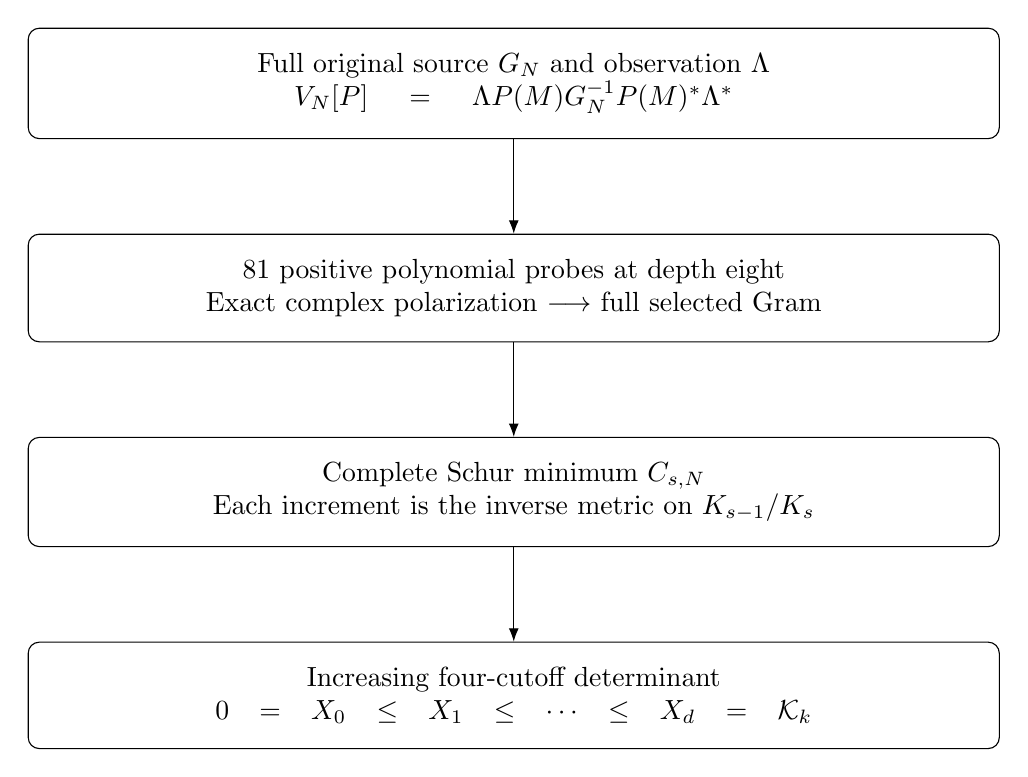
\begin{tikzpicture}[>=Latex,
 box/.style={draw,rounded corners,text width=11.7cm,align=center,inner sep=9pt}]
\node[box](a){Full original source $G_N$ and observation $\Lambda$\\
 $V_N[P]=\Lambda P(M)G_N^{-1}P(M)^*\Lambda^*$};
\node[box,below=12mm of a](b){81 positive polynomial probes at depth eight\\
 Exact complex polarization $\longrightarrow$ full selected Gram};
\node[box,below=12mm of b](c){Complete Schur minimum $C_{s,N}$\\
 Each increment is the inverse metric on $K_{s-1}/K_s$};
\node[box,below=12mm of c](d){Increasing four-cutoff determinant\\
 $0=X_0\le X_1\le\cdots\le X_d=\mathcal K_k$};
\draw[->](a)--(b);\draw[->](b)--(c);\draw[->](c)--(d);
\end{tikzpicture}
\caption{All arrows are exact maps in AP4--18. The rank of a layer specifies
its dimension; its displayed original quotient metric supplies the value.
Every nonnegative increment is bounded by $2(t_{s-1}-t_s)E_k$.
The full source estimate is inherited with its original human-source
citations from 021 BD11.}
\end{figure}
\[
 0\le\mathcal K_k-X_8\le256E_k,\qquad
 E_k=2\log C_{\rm rem}+\log(u_k/\ell_k)=O_h(q).
\]
\clearpage
\section*{The terminal metric correction remains in the original source}
\addcontentsline{toc}{section}{The terminal metric correction remains in the original source}
After eliminating only the long hidden coordinates, retain the complete
metric on the short ambient coordinates and long terminal coordinates:
\[
 G^{(1)}=\begin{pmatrix}A&B\\B^*&C\end{pmatrix}>0.
\]
\begin{figure}[H]\centering
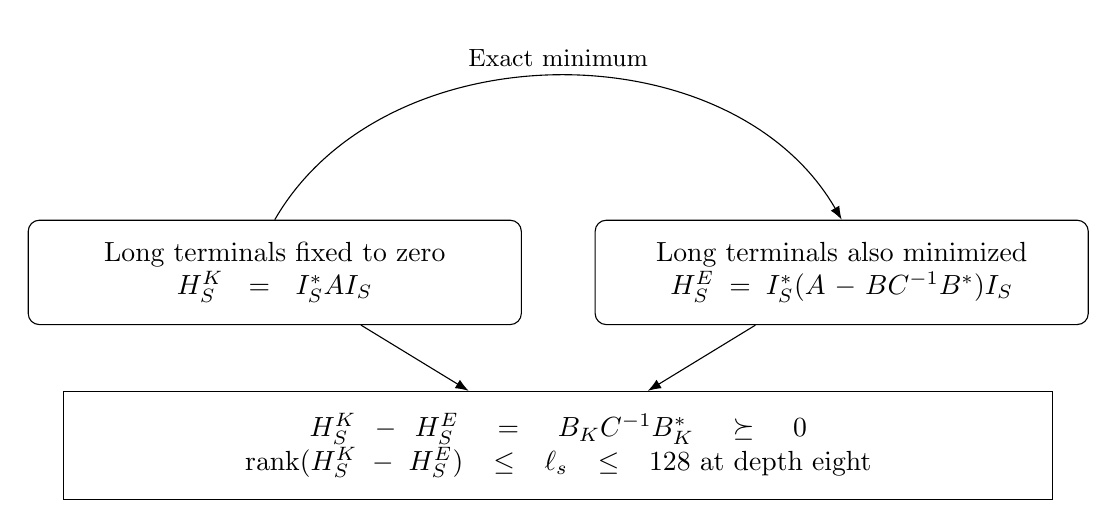
\begin{tikzpicture}[>=Latex,box/.style={draw,rounded corners,align=center,text width=5.7cm,inner sep=8pt}]
\node[box](a)at(0,0){Long terminals fixed to zero\\
 $H_S^K=I_S^*AI_S$};
\node[box](b)at(7.2,0){Long terminals also minimized\\
 $H_S^E=I_S^*(A-BC^{-1}B^*)I_S$};
 \draw[->](a.north) to[out=60,in=120] node[above,font=\small]{Exact minimum} (b.north);
\node[draw,align=center,text width=12cm,inner sep=8pt](c)at(3.6,-2.2)
 {$H_S^K-H_S^E=B_KC^{-1}B_K^*\succeq0$\\
 $\operatorname{rank}(H_S^K-H_S^E)\le\ell_s\le128$ at depth eight};
\draw[->](a)--(c);\draw[->](b)--(c);
\end{tikzpicture}
\caption{PEN17--20 prove the exact metric correction. $B_K=I_S^*B$,
and $\ell_s$ counts complete long chains. The two minima retain different
terminal constraints; the formula gives their connecting map. Their
four-cutoff log-determinant difference has absolute value at most
$2\ell_sE_k$, but need not be nonnegative.}
\end{figure}
In the complete nested auxiliary example of PEN9,
$H_S^K=1$ at every cutoff, while $H_S^E$ is $3/4$ at the two low
cutoffs and $1/2$ at the two high cutoffs. Hence
\[
 \mathcal R\log\det H_K-\mathcal R\log\det H_S^E
 =-2\log(3/2)<0.
\]
The source is positive and nested in this example. The negative return
is caused by the specified metric correction, not by a missing positivity
assumption. These are auxiliary values, not a native period evaluation.
\clearpage

\clearpage
\section*{A tighter interval from the same four kernel masses}
\addcontentsline{toc}{section}{A tighter interval from the same four kernel masses}
For the complete auxiliary fixture in KM30, the original kernel angle is
$\Gamma=1/6$, and the exact common-frame mass is
\[
 W(\sigma)=6+\frac{27}{50}\frac{\sigma^2}{(1+2\sigma/5)^2}.
\]
Use $R_3(\sigma)=W(\sigma)/21-4W(\sigma/2)/7+32W(\sigma/4)/21$.
The old upper endpoint is $R_3(\sigma/2)$; the new one subtracts the
proved lower-contraction term. The lower endpoint is unchanged.
\begin{figure}[H]\centering
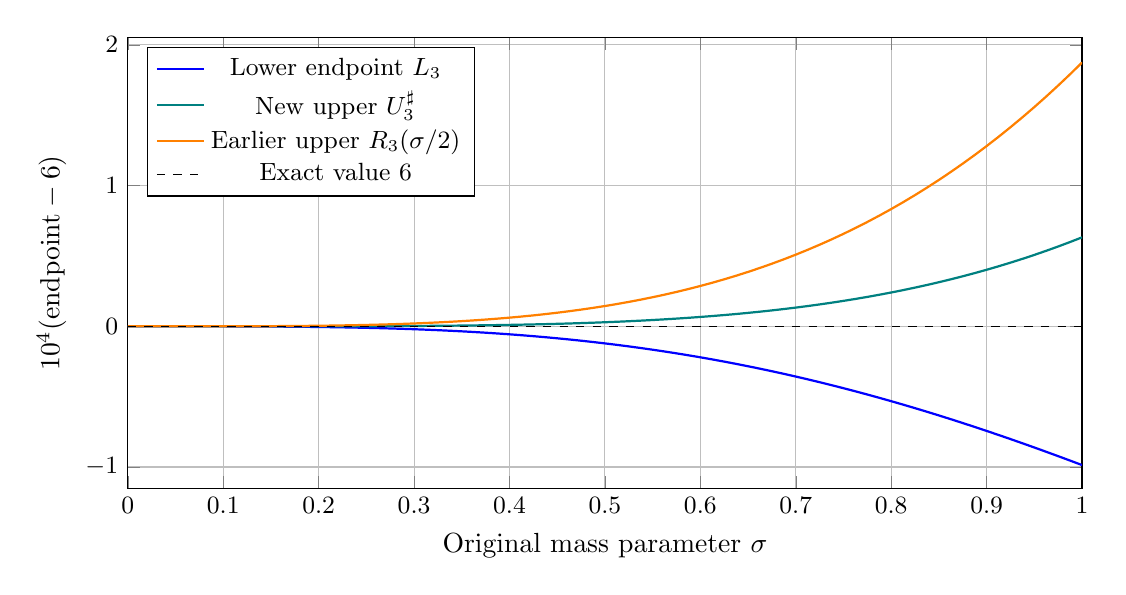
\begin{tikzpicture}
\begin{axis}[width=13.7cm,height=7.3cm,xlabel={Original mass parameter $\sigma$},
ylabel={$10^4(\text{endpoint}-6)$},xmin=0,xmax=1,ymin=-1.15,ymax=2.05,
grid=major,legend style={at={(0.02,.98)},anchor=north west,font=\small},
tick label style={font=\small}]
\addplot[blue,thick] coordinates {(0.00000000,0.0000000000) (0.01250000,-0.0000000905) (0.02500000,-0.0000014234) (0.03750000,-0.0000070859) (0.05000000,-0.0000220227) (0.06250000,-0.0000528734) (0.07500000,-0.0001078190) (0.08750000,-0.0001964369) (0.10000000,-0.0003295626) (0.11250000,-0.0005191603) (0.12500000,-0.0007781998) (0.13750000,-0.0011205400) (0.15000000,-0.0015608195) (0.16250000,-0.0021143527) (0.17500000,-0.0027970324) (0.18750000,-0.0036252373) (0.20000000,-0.0046157449) (0.21250000,-0.0057856503) (0.22500000,-0.0071522880) (0.23750000,-0.0087331604) (0.25000000,-0.0105458690) (0.26250000,-0.0126080502) (0.27500000,-0.0149373156) (0.28750000,-0.0175511953) (0.30000000,-0.0204670848) (0.31250000,-0.0237021961) (0.32500000,-0.0272735107) (0.33750000,-0.0311977368) (0.35000000,-0.0354912690) (0.36250000,-0.0401701507) (0.37500000,-0.0452500388) (0.38750000,-0.0507461718) (0.40000000,-0.0566733397) (0.41250000,-0.0630458558) (0.42500000,-0.0698775313) (0.43750000,-0.0771816519) (0.45000000,-0.0849709556) (0.46250000,-0.0932576136) (0.47500000,-0.1020532113) (0.48750000,-0.1113687327) (0.50000000,-0.1212145450) (0.51250000,-0.1316003855) (0.52500000,-0.1425353494) (0.53750000,-0.1540278793) (0.55000000,-0.1660857561) (0.56250000,-0.1787160901) (0.57500000,-0.1919253150) (0.58750000,-0.2057191810) (0.60000000,-0.2201027507) (0.61250000,-0.2350803944) (0.62500000,-0.2506557876) (0.63750000,-0.2668319086) (0.65000000,-0.2836110371) (0.66250000,-0.3009947540) (0.67500000,-0.3189839407) (0.68750000,-0.3375787807) (0.70000000,-0.3567787607) (0.71250000,-0.3765826727) (0.72500000,-0.3969886167) (0.73750000,-0.4179940037) (0.75000000,-0.4395955595) (0.76250000,-0.4617893288) (0.77500000,-0.4845706798) (0.78750000,-0.5079343091) (0.80000000,-0.5318742472) (0.81250000,-0.5563838641) (0.82500000,-0.5814558755) (0.83750000,-0.6070823491) (0.85000000,-0.6332547112) (0.86250000,-0.6599637540) (0.87500000,-0.6871996422) (0.88750000,-0.7149519209) (0.90000000,-0.7432095231) (0.91250000,-0.7719607776) (0.92500000,-0.8011934167) (0.93750000,-0.8308945847) (0.95000000,-0.8610508461) (0.96250000,-0.8916481939) (0.97500000,-0.9226720586) (0.98750000,-0.9541073163) (1.00000000,-0.9859382979)};
\addlegendentry{Lower endpoint $L_3$}
\addplot[teal,thick] coordinates {(0.00000000,0.0000000000) (0.01250000,0.0000000004) (0.02500000,0.0000000137) (0.03750000,0.0000001031) (0.05000000,0.0000004295) (0.06250000,0.0000012958) (0.07500000,0.0000031877) (0.08750000,0.0000068114) (0.10000000,0.0000131295) (0.11250000,0.0000233926) (0.12500000,0.0000391699) (0.13750000,0.0000623762) (0.15000000,0.0000952978) (0.16250000,0.0001406149) (0.17500000,0.0002014234) (0.18750000,0.0002812538) (0.20000000,0.0003840883) (0.21250000,0.0005143770) (0.22500000,0.0006770517) (0.23750000,0.0008775383) (0.25000000,0.0011217682) (0.26250000,0.0014161878) (0.27500000,0.0017677670) (0.28750000,0.0021840067) (0.30000000,0.0026729442) (0.31250000,0.0032431593) (0.32500000,0.0039037773) (0.33750000,0.0046644727) (0.35000000,0.0055354712) (0.36250000,0.0065275510) (0.37500000,0.0076520434) (0.38750000,0.0089208325) (0.40000000,0.0103463546) (0.41250000,0.0119415965) (0.42500000,0.0137200931) (0.43750000,0.0156959251) (0.45000000,0.0178837156) (0.46250000,0.0202986265) (0.47500000,0.0229563538) (0.48750000,0.0258731237) (0.50000000,0.0290656870) (0.51250000,0.0325513138) (0.52500000,0.0363477882) (0.53750000,0.0404734015) (0.55000000,0.0449469465) (0.56250000,0.0497877105) (0.57500000,0.0550154685) (0.58750000,0.0606504761) (0.60000000,0.0667134624) (0.61250000,0.0732256220) (0.62500000,0.0802086080) (0.63750000,0.0876845236) (0.65000000,0.0956759144) (0.66250000,0.1042057603) (0.67500000,0.1132974672) (0.68750000,0.1229748589) (0.70000000,0.1332621687) (0.71250000,0.1441840308) (0.72500000,0.1557654718) (0.73750000,0.1680319023) (0.75000000,0.1810091084) (0.76250000,0.1947232429) (0.77500000,0.2092008165) (0.78750000,0.2244686898) (0.80000000,0.2405540638) (0.81250000,0.2574844720) (0.82500000,0.2752877713) (0.83750000,0.2939921337) (0.85000000,0.3136260374) (0.86250000,0.3342182586) (0.87500000,0.3557978628) (0.88750000,0.3783941961) (0.90000000,0.4020368772) (0.91250000,0.4267557889) (0.92500000,0.4525810695) (0.93750000,0.4795431049) (0.95000000,0.5076725200) (0.96250000,0.5370001710) (0.97500000,0.5675571372) (0.98750000,0.5993747127) (1.00000000,0.6324843987)};
\addlegendentry{New upper $U_3^\sharp$}
\addplot[orange,thick] coordinates {(0.00000000,0.0000000000) (0.01250000,0.0000000702) (0.02500000,0.0000011169) (0.03750000,0.0000056218) (0.05000000,0.0000176650) (0.06250000,0.0000428788) (0.07500000,0.0000884018) (0.08750000,0.0001628347) (0.10000000,0.0002761966) (0.11250000,0.0004398827) (0.12500000,0.0006666227) (0.13750000,0.0009704403) (0.15000000,0.0013666140) (0.16250000,0.0018716378) (0.17500000,0.0025031842) (0.18750000,0.0032800665) (0.20000000,0.0042222037) (0.21250000,0.0053505847) (0.22500000,0.0066872340) (0.23750000,0.0082551786) (0.25000000,0.0100784146) (0.26250000,0.0121818757) (0.27500000,0.0145914019) (0.28750000,0.0173337086) (0.30000000,0.0204363573) (0.31250000,0.0239277262) (0.32500000,0.0278369817) (0.33750000,0.0321940510) (0.35000000,0.0370295948) (0.36250000,0.0423749807) (0.37500000,0.0482622576) (0.38750000,0.0547241304) (0.40000000,0.0617939355) (0.41250000,0.0695056162) (0.42500000,0.0778937002) (0.43750000,0.0869932757) (0.45000000,0.0968399697) (0.46250000,0.1074699258) (0.47500000,0.1189197832) (0.48750000,0.1312266555) (0.50000000,0.1444281108) (0.51250000,0.1585621514) (0.52500000,0.1736671951) (0.53750000,0.1897820557) (0.55000000,0.2069459250) (0.56250000,0.2251983545) (0.57500000,0.2445792383) (0.58750000,0.2651287955) (0.60000000,0.2868875537) (0.61250000,0.3098963328) (0.62500000,0.3341962291) (0.63750000,0.3598285997) (0.65000000,0.3868350473) (0.66250000,0.4152574057) (0.67500000,0.4451377252) (0.68750000,0.4765182588) (0.70000000,0.5094414481) (0.71250000,0.5439499104) (0.72500000,0.5800864257) (0.73750000,0.6178939235) (0.75000000,0.6574154710) (0.76250000,0.6986942609) (0.77500000,0.7417735994) (0.78750000,0.7866968952) (0.80000000,0.8335076477) (0.81250000,0.8822494371) (0.82500000,0.9329659126) (0.83750000,0.9857007833) (0.85000000,1.0404978072) (0.86250000,1.0974007819) (0.87500000,1.1564535350) (0.88750000,1.2176999145) (0.90000000,1.2811837805) (0.91250000,1.3469489953) (0.92500000,1.4150394161) (0.93750000,1.4854988854) (0.95000000,1.5583712240) (0.96250000,1.6337002222) (0.97500000,1.7115296327) (0.98750000,1.7919031629) (1.00000000,1.8748644676)};
\addlegendentry{Earlier upper $R_3(\sigma/2)$}
\addplot[black,dashed,domain=0:1]{0};\addlegendentry{Exact value $6$}
\end{axis}
\end{tikzpicture}
\caption{The same four scales $\sigma,\sigma/2,\sigma/4,\sigma/8$ give all
three endpoints. KM20--25 prove their order at every $0<\sigma\le1$.
Plot coordinates are generated from exact rational expressions at 81
rational parameter values, rounded only for display. The vertical factor
$10^4$ magnifies the error; it does not rescale the underlying source metric.
These are the stated auxiliary matrices, not a native xi-packet value.}
\end{figure}
At $\sigma=1$ the strengthened exact interval is
\[
 \frac{1572060375}{262014368}
 <6<
 \frac{284595}{47432}
 <\frac{7968825}{1328096}.
\]

\clearpage\part{Positive probes and increasing depth determinants}
\section{Positive arithmetic probes and the increasing original determinant}\label{positive-arithmetic-probes-and-the-increasing-original-determinant}

Result SZ-20260922-022, probe derivation. The incoming arithmetic-probe manuscript supplies the finite polarization construction. This proof establishes its maps completely, strengthens its finite-error constant, evaluates the optimal positive regularizer for the resulting error bound, and derives a positive, telescoping determinant at every original observation depth. No native period-dependent value is assigned by a dimension count.

The exact predecessor is \href{https://github.com/KokunoYumeto/zeta-function-research-reader/blob/e40b46fde72c245dd79ef5691f59c21d6cbf0c75/workbenches/splitzero-tandem/continuations/20260922-original-observation-recovery/BOUNDED_DEGREE_PROOFS.md}{BD1--31, original arithmetic observation and whole-source estimate}, \href{https://github.com/KokunoYumeto/zeta-function-research-reader/blob/e40b46fde72c245dd79ef5691f59c21d6cbf0c75/workbenches/splitzero-tandem/continuations/20260922-original-observation-recovery/MATRIX_RECOVERY_PROOFS.md}{MR1--29, original matrix recovery}, and \href{https://github.com/KokunoYumeto/zeta-function-research-reader/blob/e40b46fde72c245dd79ef5691f59c21d6cbf0c75/workbenches/splitzero-tandem/continuations/20260922-original-observation-recovery/SCALAR_RECOVERY_PROOFS.md}{SD1--54, scalar recovery}. The public files are pinned to the verified 021 proof commit.

\subsection{AP1. Original spaces and source}\label{ap1.-original-spaces-and-source}

Retain the actual admitted period and hypothetical simple quartet of the preceding programme proofs. Thus \(q=(k+1)^2\), \(k\equiv1\pmod4\), \(k\ge17\), \(0<\delta<1/2\), and the actual quartet satisfies the finite-height guard in BD1. In the original physical coordinate, \[
 Q_k(y)=\prod_{a,b=0}^k\bigl(y-(2b-k)\gamma+i(2a-k)\delta\bigr),
 \quad E=\mathbb C[y]/(Q_k),\quad M[p]=[yp].
\] The physical arithmetic operator is \(kI/2+iM\). The original onto observation is \(\Lambda:E\to B\), its kernel is \(K\), and its fixed frame is \(I_K:\mathbb C^m\to K\), where \(m=8k-16\), \(n=q-m\). For each of the four cutoffs \(N=q-1,q,2q-1,2q\), use the attained source metric \(G_N>0\), including the complete original source measure and its mass. Put \[
 Q_N=(\Lambda G_N^{-1}\Lambda^*)^{-1},\quad
 L_N=G_N^{-1}\Lambda^*Q_N,\quad H_{K,N}=I_K^*G_NI_K.
 \tag{AP1}
\] All stars refer to conjugate transpose in the indicated coefficient frames. Write \[
 \mathcal R f=f_{q-1}+f_q-f_{2q-1}-f_{2q},\qquad
 \mathcal K_k=\mathcal R\log\det H_{K,N}.
\] The complete source inequality needed below is the explicitly proved BD21: \[
 e^{-E_k}G_{q-1}\preceq G_N\preceq G_{q-1},
 \quad E_k=2\log C_{\rm rem}+\log(u_k/\ell_k)=O_h(q).
 \tag{AP2}
\] Here \(r=k\sqrt{\delta^2+\gamma^2}/q\), \(t=\max(1,r)\), \[
 C_{\rm rem}=(2\pi)^{1/4}2^q
 \left(1+(q+1)[4t(1+r)]^q\right)
 \frac{(2q+1)11^{2q}e^{\pi q}}{\sqrt{C_Lq}},
 \qquad C_L=\frac{\pi}{\Gamma(3/4)^2}.
\] The bounds \(\ell_k,u_k\) apply to every polynomial through degree \(2q\) in the original measure. The proof of AP2, including the Gamma mass and every root, is retained in full in the predecessor BD11. We use that independently derived constant instead of assuming the different unevaluated remainder constant in the new incoming text. Source nesting gives \(G_{N'}\preceq G_N\) whenever \(N'\ge N\).

BD1--3 prove, with the actual corner and period guards, \[
 K_s=\bigcap_{j=0}^s\ker(\Lambda M^j),\quad
 t_s=\dim K_s,\quad t_0=m,\quad t_8\le128,\quad K_d=0,\ d\le80.
 \tag{AP3}
\] No conductor kernel is substituted for the kernel of the complete observation.

\subsection{AP2. Every specified positive probe is an original operator}\label{ap2.-every-specified-positive-probe-is-an-original-operator}

For a polynomial \(P\), define \[
 V_N[P]=\Lambda P(M)G_N^{-1}P(M)^*\Lambda^*.
 \tag{AP4}
\] All roots of \(Q_k\) have modulus at least \(\sqrt{\delta^2+\gamma^2}>2\), since \(k\) is odd. For \(0\le i<j\le s\), the polynomials \[
 y^i,\qquad y^i+y^j,\qquad y^i+iy^j
 \tag{AP5}
\] are nonzero at every original root. Indeed their possible additional zeros satisfy \(|y|=1\). Bezout division therefore gives a unique residue polynomial for \(P^{-1}\) modulo the full \(Q_k\). It defines \(T_P=P(M)^{-1}\) on the same \(E\), with no change of source degree, and \[
 V_N[P]=\Lambda(T_P^*G_NT_P)^{-1}\Lambda^*.
 \tag{AP6}
\] This follows by multiplying the proposed inverse \(P(M)G_N^{-1}P(M)^*\) on both sides by \(T_P^*G_NT_P\).

There is also an exact energy map. Suppressing \(N\), let \(P^\dagger=G^{-1}P(M)^*G\). Since \(GL=\Lambda^*Q\), \[
 L^*G(P^\dagger)^\dagger P^\dagger L
 =L^*GP(M)G^{-1}P(M)^*GL
 =QV[P]Q. \tag{AP7}
\] Both quotient factors remain. This proves the relation between the reciprocal-word inverse energy and the full adjoint-word energy before any compression.

\subsection{AP3. Exact polarization and selected source minimum}\label{ap3.-exact-polarization-and-selected-source-minimum}

Set \(S_{ij}=\Lambda M^iG^{-1}(M^*)^j\Lambda^*\), and let \(D_i=V[y^i]\). Expansion of the two mixed probes gives \[
 A_{ij}=V[y^i+y^j]-D_i-D_j=S_{ij}+S_{ji},
\] \[
 B_{ij}=V[y^i+iy^j]-D_i-D_j=-iS_{ij}+iS_{ji}.
\] Consequently \[
 S_{ii}=D_i,\quad S_{ij}=\tfrac12(A_{ij}+iB_{ij}),\quad S_{ji}=S_{ij}^*.
 \tag{AP8}
\] There are \((s+1)^2\) positive probes. This is the classical complex polarization identity applied to these exact arithmetic words; the identity itself is not claimed as new.

The whole matrix equals \[
 \mathcal S_{s,N}=\mathcal O_sG_N^{-1}\mathcal O_s^*,
 \qquad\mathcal O_s=\operatorname{col}_{j=0}^s(\Lambda M^j). \tag{AP9}
\] Start with every row of \(\Lambda\). At each successive depth, append independent scalar rows from \(\Lambda M^s\), preserving all earlier selected rows. Let \(r_s=m-t_s\). The selected map has full row rank \(n+r_s\). Its Gram is positive definite. The complete Schur complement of its initial \(Q_N^{-1}\) block is \[
 C_{s,N}=J_s H_{K,N}^{-1}J_s^*, \tag{AP10}
\] where \(J_s\) consists of the selected rows of \(\Lambda M^jI_K\), \(j\ge1\).

For a direct proof of the source identity used here, the square matrix \(U=[L,I_K]\) is invertible: applying \(\Lambda\) shows that its two summands intersect trivially and span \(E\). Its Gram is \(\operatorname{diag}(Q,H_K)\), because \(\Lambda L=I\), \(L^*GL=Q\), and \(L^*GI_K=0\). Inverting the Gram and transporting it back gives \[
 G^{-1}=LQ^{-1}L^*+I_KH_K^{-1}I_K^*.
\] Its first term is \(G^{-1}\Lambda^*Q\Lambda G^{-1}\). Applying the selected rows on both sides proves AP10, including every cross block.

Choose fixed \(P_1,P_0\) with \(J_sP_1=I\) and \(I_KP_0\) a basis of \(K_s\). In the basis \([P_1,P_0]\), AP10 is the upper principal block of the inverse of \(H_K\). Inversion by completing the square gives \[
 \det H_K
 =\frac{\det(P_0^*H_KP_0)}{|\det[P_1,P_0]|^2\det C_s}.
\] The fixed coefficient determinant cancels under the four original signs. Thus \[
 X_s:=-\mathcal R\log\det C_{s,N},\quad
 Z_s:=\mathcal R\log\det(P_0^*H_{K,N}P_0),\quad
 \mathcal K_k=X_s+Z_s. \tag{AP11}
\] For \(s=0\), the determinant of the empty \(C_0\) is one and \(X_0=0\). At \(s=d\), \(Z_d=0\) and \(J_d\) is square: \[
 H_{K,N}^{-1}=J_d^{-1}C_{d,N}J_d^{-*}. \tag{AP12}
\] If \(\mathcal B_d\mathcal O_d=I\), AP9 also gives \(G_N^{-1}=\mathcal B_d\mathcal S_{d,N}\mathcal B_d^*\).

Restricting AP2 and using source nesting at the paired cutoffs proves \[
 0\le Z_s\le2t_sE_k.
 \tag{AP13}
\] Each low-to-high determinant ratio lies between one and \(e^{t_sE_k}\). At depth eight there are 81 positive probes and \(0\le\mathcal K_k-X_8\le256E_k=O_h(q)\). At depth at most80, 6561 probes suffice for exact full recovery. The arithmetic values of these matrices are still required.

\subsection{AP4. New positive increments at every depth}\label{ap4.-new-positive-increments-at-every-depth}

Let \(b_s=t_{s-1}-t_s=r_s-r_{s-1}\). If \(b_s=0\), put \(D_{s,N}\) equal to the empty matrix. Otherwise take the complete Schur complement of \(C_{s-1,N}\) in the successively selected \(C_{s,N}\): \[
 D_{s,N}=C_{s,N}^{\rm new,new}
 -C_{s,N}^{\rm new,old}C_{s-1,N}^{-1}C_{s,N}^{\rm old,new}.
 \tag{AP14}
\] Every \(D_{s,N}\) is positive definite. Completing the square proves \(\det C_s=\det C_{s-1}\det D_s\). Therefore \[
 X_s-X_{s-1}=-\mathcal R\log\det D_{s,N}. \tag{AP15}
\] These are the actual original observation innovations; no chain block is declared invariant under \(M\).

Here is their source metric meaning. After all prior observation rows are fixed, their common nullspace is \(K_{s-1}\). Apply the same identity used in AP10 to that complete prior observation map. It shows that \(D_s\) is the covariance of the new rows restricted to \(K_{s-1}\), in the inverse of its original restricted metric. These new rows have nullspace \(K_s\). Consequently \(D_s^{-1}\) is exactly the attained quotient metric on \(K_{s-1}/K_s\), in the fixed new-row coordinate frame.

For explicit connecting maps, let \(I_{s-1}\) be a fixed frame of \(K_{s-1}\), \(F_s\) the new observation rows restricted to that frame, and \(H_{s-1,N}=I_{s-1}^*G_NI_{s-1}\). Then \[
 D_{s,N}=F_sH_{s-1,N}^{-1}F_s^*,\qquad
 L_{s,N}=H_{s-1,N}^{-1}F_s^*D_{s,N}^{-1},\quad F_sL_{s,N}=I.
 \tag{AP16}
\] The lift \(L_{s,N}\) is orthogonal to \(\ker F_s\), so its energy is \(D_{s,N}^{-1}\). This proves the exact quotient assertion.

Restrictions and minima preserve both inequalities in AP2 and preserve source nesting. Applying the same two paired determinant comparisons to this rank-\(b_s\) quotient gives \[
 0\le X_s-X_{s-1}\le2b_sE_k. \tag{AP17}
\] In particular, \[
 0=X_0\le X_1\le\cdots\le X_d=\mathcal K_k,\qquad
 \mathcal K_k=\sum_{s=1}^d\bigl[-\mathcal R\log\det D_{s,N}\bigr].
 \tag{AP18}
\] Summing only after depth \(s\) gives AP13 again because \(\sum_{j>s}b_j=t_s\). This proves a positive decomposition of the original signed return; it is stronger than an error estimate for one truncation. It does not determine the values of the positive increments.

The dimensions are intrinsic: BD6 gives \(b_s=\#\{a:\epsilon_a\ge s\}\) for the actual observation-chain lengths. AP16 supplies the metric on each such quotient and therefore the data omitted by the integer multiplicity alone. In particular \(b_1\ge k-18\) on the proved domain and \(\sum_{s>8}b_s\le128\).

\subsection{AP5. Data size and a stronger finite-error constant}\label{ap5.-data-size-and-a-stronger-finite-error-constant}

Let \(r_i\) be the number of selected new rows from level \(i\). With the original \(Q_N^{-1}\) known, diagonal probes need at most \(n\sum r_i=nr_s\) complex entries; pairs with level zero need \(2nr_s\); other pairs need \(2\sum_{i<j}r_ir_j\). The required diagonal subtractions are already included, with the opposite blocks supplied by Hermitian symmetry. Thus \[
 \text{additional complex entries}\le3nr_s+r_s^2=O(kq). \tag{AP19}
\] The baseline's \(n^2\) real entries and the precision of every requested value remain part of the calculation.

Suppose each supplied covariance has operator error at most \(\eta\), measured in one fixed observed coefficient norm. Replace it by its Hermitian part, which does not increase this error. In AP8 the off-diagonal error can be collected as \[
 \tfrac12\left(E_{ij}^{+}+iE_{ij}^{\,i}-(1+i)(E_i+E_j)\right).
\] Its norm is at most \((1+\sqrt2)\eta\), improving the incoming \(3\eta\) bound. The diagonal error is at most \(\eta\). For block vectors use the scalar matrix with diagonal1 and off-diagonal \(1+\sqrt2\); its largest absolute eigenvalue is \(1+s(1+\sqrt2)\). The triangle inequality followed by its quadratic-form bound proves \[
 \|\widehat{\mathcal S}_s-\mathcal S_s\|
 \le a_s\eta,\qquad a_s=1+s(1+\sqrt2). \tag{AP20}
\] A scalar-row principal selection cannot enlarge the bound.

If the actual selected Gram has lower eigenvalue bound \(h_N> a_s\eta\), put \(\varepsilon_N=a_s\eta/h_N\). Then its full relative bounds are \(1-\varepsilon_N\) and \(1+\varepsilon_N\). Minimizing each bounding form over the same first-coordinate fibre transfers those bounds to \(C_{s,N}\). For \(\varepsilon_N\le\varepsilon<1\) at all cutoffs, \[
 |\widehat X_s-X_s|\le
 e_s:=2r_s\log\frac{1+\varepsilon}{1-\varepsilon}. \tag{AP21}
\] Combining with AP13 gives \[
 \widehat X_s-e_s\le\mathcal K_k
 \le\widehat X_s+e_s+2t_sE_k. \tag{AP22}
\] These intervals can be intersected over all computed depths. The certified lower endpoint can additionally be replaced by its maximum with zero. The upper endpoint can be replaced by the minimum of all the displayed upper endpoints. AP18 proves validity without assuming independent errors or adding the same source remainder repeatedly.

A directly computable eigenvalue floor is \(\lambda_{\min}(\widehat{\mathcal S}^{\rm sel}_s)-a_s\eta\), when positive, since the Rayleigh quotient changes by at most \(a_s\eta\). Another is \(\sigma_{\min}(\mathcal O_s^{\rm sel})^2/\lambda_{\max}(G_N)\). These are numerical margins of the actual matrices, never consequences of rank alone.

\subsection{AP6. New optimal positive regularizer for the certified error}\label{ap6.-new-optimal-positive-regularizer-for-the-certified-error}

For an invertible polynomial probe keep the original response \[
 Y_P(z)=\Lambda z(zI+G^{-1}T_P^*GT_P)^{-1}L,\quad z>0.
\] Multiplication by \(G\) and \(GL=\Lambda^*Q\) proves \[
 \Sigma_P(z)=z^{-1}Y_P(z)Q^{-1}
 =\Lambda(T_P^*GT_P+zG)^{-1}\Lambda^*. \tag{AP23}
\] Let \(a\ge\|P(M)\|_G^2\), \(b\ge\|V[P]\|\), both positive certified finite numbers. For \(x=P(M)y\), the norm inequality gives \(y^*Gy\ge a^{-1}x^*Gx\). Hence \(T_P^*GT_P\succeq a^{-1}G\). Adding \(zG\), inverting, and applying \(\Lambda\) proves \[
 (1+za)^{-1}V[P]\preceq\Sigma_P(z)\preceq V[P].
\] If the measured response has operator error at most \(\eta_P\) and the supplied \(Q^{-1}\) is exact, set \(c=\eta_P\|Q^{-1}\|\). After Hermitian projection, a full error bound is \[
 \|\widehat\Sigma_P(z)-V[P]\|
 \le f(z):=\frac{baz}{1+az}+\frac c z. \tag{AP24}
\] The first term is the exact consequence of the relative bias, stronger than \(baz\). The second retains the observed response amplification.

For \(c>0\) and \(ac<b\), let \(\tau=\sqrt{ac/b}\in(0,1)\). Differentiating AP24 gives \[
 z_*=\frac{\tau}{a(1-\tau)},\qquad
 \min_{z>0}f(z)=b(2\tau-\tau^2)=2\sqrt{abc}-ac. \tag{AP25}
\] Indeed \(f'(z)=ba/(1+az)^2-c/z^2\), which changes sign exactly once at \(z_*\). If \(ac\ge b\), this derivative is negative and the infimum is \(b\) as \(z\to\infty\). For \(c=0\), the infimum is zero as \(z\downarrow0\). Those limiting cases do not assert a finite regularizer achieving the infimum.

For a requested covariance error \(0<\eta<b\), the sufficient and exact threshold for this bound is \[
 \eta_P\le
 \frac{b}{a\|Q^{-1}\|}
 \left(1-\sqrt{1-\eta/b}\right)^2. \tag{AP26}
\] Use \(z_*\) with the actual \(c\), or any positive \(z\) whose AP24 value is below the target. This evaluates the best tradeoff in the specified certified bound. It makes no assertion that its constants are the actual worst-case errors of all native probes.

The inverse quotient error has an explicit place in this bound. If \(\|\widehat D-Q^{-1}\|\le\xi\), \(\|\widehat Y-Y\|\le\eta_P\), and \(\|Y\|\le y_0\), expansion of \(\widehat Y\widehat D-YQ^{-1}\) bounds its norm by \[
 c=\eta_P\|Q^{-1}\|+(y_0+\eta_P)\xi. \tag{AP26a}
\] AP24--25 hold with this \(c\). One uniform valid value is \(y_0=\sqrt{\|Q\|\|Q^{-1}\|}\): the response is a positive contraction in the \(Q\) metric, because \(Q^{1/2}YQ^{-1/2}\) is the compression of \(z(z+H)^{-1}\) by the original \(G\)-isometric section \(LQ^{-1/2}\). Its Euclidean norm is therefore at most the displayed similarity bound. This proves the complete amplification of both measured factors.

\subsection{AP7. Centered current with the actual quotient uncertainty}\label{ap7.-centered-current-with-the-actual-quotient-uncertainty}

Put \(M_B=\Lambda ML=S_{10}Q\). The physical centered action is \(iM_B\). In the original output frame its real current is \[
 \Phi(b)=i b^*(QM_B-M_B^*Q)b
 =b^*Q\,i(S_{10}-S_{01})Qb. \tag{AP27}
\] The two positive covariances give \[
 T_c=\tfrac12\bigl(V[1+iy]-V[1-iy]\bigr)
 =i(S_{10}-S_{01}). \tag{AP28}
\] This is the same complete current as the polynomial-gauge formula BD29, since both equal the first expression in AP27. Thus the connecting map includes its derivative correction automatically. It does not substitute for other cross-pairings in BD31.

With exact \(Q,b\), two covariance errors of norm at most \(\eta\) imply \[
 |\widehat\Phi-\Phi|\le\eta\|Qb\|^2.
\] Now also allow a Hermitian quotient estimate with \[
 \widehat Q=Q^{1/2}(I+E)Q^{1/2},\quad\|E\|\le\varepsilon,
 \qquad \|Q^{1/2}(\widehat T_c-T_c)Q^{1/2}\|\le\zeta.
\] These are measured errors in the original quotient geometry. Put \(A=Q^{1/2}T_cQ^{1/2}\), \(y=Q^{1/2}b\). Then \[
 \widehat\Phi=y^*(I+E)(A+\Delta A)(I+E)y,\quad \Phi=y^*Ay.
\] Expanding every term and using the operator norm gives the complete bound \[
 |\widehat\Phi-\Phi|
 \le\left[(2\varepsilon+\varepsilon^2)\|A\|
 +(1+\varepsilon)^2\zeta\right]\,b^*Qb. \tag{AP29}
\] This keeps both quotient factors and their cross term. The vector \(b\) here is the fixed original observed class. It is not replaced by a newly minimized vector at each probe.

If its supplied value is also approximate, set \(\rho=\|Q^{1/2}(\widehat b-b)\|\), \(v=\sqrt{b^*Qb}\), and let \(e_A\) be the bracket in AP29. The same expansion gives \[
 |\widehat\Phi(\widehat b)-\Phi(b)|
 \le e_Av^2+(2\rho v+\rho^2)(1+\varepsilon)^2(\|A\|+\zeta).
 \tag{AP30}
\] Indeed the difference between the quadratic forms of the computed Hermitian matrix at \(y\) and \(y+\Delta y\) is at most its norm times \(2\|\Delta y\|\|y\|+\|\Delta y\|^2\). Thus the acquisition error of the original class is also retained.

\subsection{AP8. Exact verification and attribution}\label{ap8.-exact-verification-and-attribution}

The checker constructs a four-dimensional companion action with roots \(2,3,4,5\), one original observation row, a nonidentity complex covariance and a positive rank-one source update at four cutoffs. The true native root grid is not identified with this example. It verifies every complex probe, the whole Schur complement, the nested determinant factorization, the quotient maps AP16, and the current before and after polarization. It also checks AP25--26 by exact algebra. A reversed imaginary phase and a raw lower-right block fail in explicit negative controls.

The incoming proof's finite-polarization and complete selected-covariance construction is retained as provenance. The new contributions here are AP17--18's increasing depth return, AP20's stronger error constant, AP25--26's evaluated regularizer and AP29's full quotient-error current bound. The original source estimate and observation-depth theorem are credited to SZ-20260922-021, BD1--3 and BD11--12, whose complete proofs accompany this continuation. Classical Schur elimination is proved above; its human-source context is Geneviève Dusson, Israel Michael Sigal and Benjamin Stamm, \href{https://arxiv.org/abs/2105.02058v1}{The Feshbach--Schur map and perturbation theory, arXiv:2105.02058v1}, Theorem1.2 and the equations labelled Fesh and QP, read in original author TeX as recorded in the predecessor.

The fixed original matrix values still determine the \(kq\) coefficient and separate current signs. The new positive filtration and finite acquisition budget specify and strengthen that calculation; they do not replace those values by ranks.

\clearpage\part{Common kernel mass and sharper determinant intervals}
\section{Fixed-kernel mass, sharp dyadic contraction, and original determinant recovery}\label{fixed-kernel-mass-sharp-dyadic-contraction-and-original-determinant-recovery}

This is an independent derivation for the 022 intake. It retains the original observation, word, source metric, zero-energy space and full kernel. The input is the complete \texttt{inputs/KERNEL\_MEMORY\_MASS.md} and Section 2 of \texttt{PROOF.md} in the supplied arithmetic-probe package. Their core mass and two-sided extrapolation statements are valid. The additional results below are the lower contraction, a tighter upper matrix using the same samples, a stronger finite defect constant, and a direct original-boundary covariance receiver. No native period value is assigned.

The finite elimination is the Feshbach--Schur construction of Geneviève Dusson, Israel Michael Sigal and Benjamin Stamm, \href{https://arxiv.org/abs/2105.02058v1}{arXiv:2105.02058v1, Theorem 1.2}, with original author TeX lines 398--489 read. The complete finite identities used here are proved below. The existing \href{https://github.com/KokunoYumeto/zeta-function-research-reader/blob/13ca9b136fcdae48df7454bd9bf99e1ef22dd03c/workbenches/splitzero-tandem/continuations/20260922-original-growth-resolvent/ORIGINAL_RESOLVENT_MEMORY_PROOFS.md}{020 exact-memory proof RM1--23} and \href{https://github.com/KokunoYumeto/zeta-function-research-reader/blob/13ca9b136fcdae48df7454bd9bf99e1ef22dd03c/workbenches/splitzero-tandem/continuations/20260922-original-growth-resolvent/RECEIVED_RESOLVENT_PROOFS.md}{original resolvent proof PR19--22} retain their attributions. The sealed 021 providers are \href{https://github.com/KokunoYumeto/zeta-function-research-reader/blob/e40b46fde72c245dd79ef5691f59c21d6cbf0c75/workbenches/splitzero-tandem/continuations/20260922-original-observation-recovery/MATRIX_RECOVERY_PROOFS.md}{MR1--29, full matrix recovery} and \href{https://github.com/KokunoYumeto/zeta-function-research-reader/blob/e40b46fde72c245dd79ef5691f59c21d6cbf0c75/workbenches/splitzero-tandem/continuations/20260922-original-observation-recovery/SCALAR_RECOVERY_PROOFS.md}{SD1--54, scalar recovery and original determinant receiver}. Their exact source identities are recorded in the ledger.

\subsection{1. Complete original spaces and the mass identity}\label{complete-original-spaces-and-the-mass-identity}

Let \(E=\mathbb C^q\), \(G=G^*>0\), and let the original onto observation be \(\Lambda:E\to B=\mathbb C^n\). Let \(I_K:\mathbb C^m\to E\) be the fixed full column frame of \(K=\ker\Lambda\), where \(m=q-n\). For the unchanged word \(T:E\to E\), set \[
\begin{gathered}
 H=G^{-1}T^*GT,\quad V=\ker T,\quad \nu=\operatorname{rank}T,\\
 Q=(\Lambda G^{-1}\Lambda^*)^{-1},\quad L=G^{-1}\Lambda^*Q,
 \quad H_K=I_K^*GI_K.
 \end{gathered}
 \tag{KM1}
\] All adjoints between physical spaces use \(G\). A star on a coordinate matrix is its conjugate transpose. The actual isometries are \(J_B=LQ^{-1/2}\), \(J_K=I_KH_K^{-1/2}\). Multiplication gives \(\Lambda L=I\), \(L^*GL=Q\), \(J_K^*GJ_K=I\), and \(J_B^*GJ_K=0\). Thus these maps give an orthogonal decomposition with inverse \([J_B,J_K]^*G\); the original \(G,Q,H_K\) have not been replaced.

Put \(Z=K\cap V\), \(t=\dim Z\), \(K_+=K\ominus_GZ\), and \(p=m-t\). Choose once a \(G\)-isometry \(J_+:\mathbb C^p\to K_+\). In a fixed frame \([I_Z,I_1]=I_KS\), the metric on \(K/Z\) is \[
 H_{\rm quot}=H_{11}-H_{01}^*H_{00}^{-1}H_{01};
 \qquad x\longmapsto I_1x-I_ZH_{00}^{-1}H_{01}x
 \tag{KM2}
\] is its isometry into \(K_+\). This follows by completing the full \(G\)-square in the \(I_Z\) coefficient. No arbitrary block of the source metric is deleted.

Define \[
 A=J_+^*GHJ_+>0,\quad C=J_+^*GHJ_B,\quad B_0=J_B^*GHJ_B,
 \quad Y(z)=Q^{1/2}\Lambda z(zI+H)^{-1}LQ^{-1/2}.
\] The zero block \(Z\) is annihilated by \(H\) and has no energy cross term. Inverting the remaining full block of \(zI+H\) gives \[
\begin{gathered}
 F(z):=zY(z)^{-1}=zI+B_0-C^*(zI+A)^{-1}C,\\
 W_B=F'(0)=I+C^*A^{-2}C,\qquad
 W_K=I+A^{-1}CC^*A^{-1}.
 \end{gathered}
 \tag{KM3}
\] These formulas follow also by solving the lower equation \((zI+A)a+Cb=0\) and substituting into the upper equation. In original observed value coordinates, \(F\) is the congruence of \(zQ\mathscr Y(z)^{-1}\), where \(\mathscr Y=\Lambda z(zI+H)^{-1}L\); its multiplication order is fixed. Sylvester elimination in \(\left(\begin{smallmatrix}I&U\\-V&I\end{smallmatrix}\right)\) proves \(\det(I+UV)=\det(I+VU)\). Consequently \(\det W_B=\det W_K\), with the distinct numbers of unit eigenvalues retained.

Write \(P=P_{V^{\perp_G}}^G\), \(H_+=H|_{V^{\perp_G}}\), and \[
 \Gamma=J_+^*GPJ_+,\quad R=PJ_+,\quad U=R\Gamma^{-1/2}.
\] Here \(0<\Gamma\preceq I_p\): \(PJ_+x=0\) would put \(J_+x\) in \(K_+\cap V=0\). Moreover \(U^*GU=I\). Put \(A_0=U^*GH_+U\). Since \(H\) annihilates \(V\), \(A=\Gamma^{1/2}A_0\Gamma^{1/2}\) and \(A^2+CC^*=\Gamma^{1/2}U^*GH_+^2U\Gamma^{1/2}\). It follows that \[
 W_K=\Gamma^{-1/2}(I+\mathcal E^*\mathcal E)\Gamma^{-1/2},
 \quad \mathcal E=(I-UU^{\dagger_G})H_+UA_0^{-1},
 \quad \operatorname{rank}\mathcal E\le d_0:=\min(p,\nu-p).
 \tag{KM4}
\] Indeed insert \(I=UU^{\dagger_G}+(I-UU^{\dagger_G})\) between the two \(H_+\) factors. This proves the mass identity including every off-diagonal positive-energy term.

For actual positive spectral bounds \(lI\preceq_G H_+\preceq_G uI\), functional calculus gives \(H_+^2\preceq(l+u)H_+-luI\). Compress by \(U\), then use \[
 (l+u)x-lu\le \frac{(l+u)^2}{4lu}x^2
 \quad\text{because}\quad
 \frac{((l+u)x-2lu)^2}{4lu}\ge0.
\] The result is \[
 \Gamma^{-1}\preceq W_K\preceq
 \frac{(l+u)^2}{4lu}\Gamma^{-1},\qquad
 0\le\log\det W_B+\log\det\Gamma
 \le d_0\log\frac{(l+u)^2}{4lu}.
 \tag{KM5}
\] The upper constant is the classical Kantorovich constant, here derived directly. To attain it, choose a unit vector in a two-dimensional positive space with eigenvalues \(l,u\), giving the \(l\)-eigenspace weight \(u/(l+u)\) and the \(u\)-eigenspace weight \(l/(l+u)\). Then its compressed energy is \(2lu/(l+u)\) and its mass ratio is exactly the displayed constant. Adding any zero component to that kernel vector supplies a prescribed angle in \((0,1]\); choosing its orthogonal-complement observation gives the complete original setup.

The memory space \(\mathcal M=\operatorname{span}\{A^jCb:0\le j<p\}\) is reducing for \(A\); its complement is annihilated by \(C^*\). For an eigenvector \(x\) in that complement, \(HJ_+x=J_+Ax\) has positive eigenvalue, so \(J_+x\in V^{\perp_G}\). Hence \(\Gamma x=x\). By spectral decomposition, \[
 \Gamma=\Gamma_{\mathcal M}\oplus I_{\mathcal M^\perp}.
 \tag{KM6}
\] The \(t\) original zero-angle directions are still \(Z\); they are not unit directions. This is the exact connection to MR8 and MR11. A memory reduction removes only unit positive angle factors and keeps the actual metric of its chosen frame.

\subsection{2. The common filtered kernel mass}\label{the-common-filtered-kernel-mass}

For \(\sigma>0\), define \(H_\sigma=H(\sigma I+H)^{-1}\). This is the energy of the specified operator \(T_\sigma=T(\sigma I+H)^{-1/2}\) in the same \(G\); it is not identified with the original polynomial word. Its zero space is \(V\), and therefore \(\Gamma\) is unchanged. The full scalar functional identity, including eigenvalue zero, gives \[
 Y_\sigma(s)=\frac{sI+Y(\sigma s/(1+s))}{1+s},\qquad s>0.
 \tag{KM7}
\] Indeed both sides on an energy \(\lambda\) equal \(s(\sigma+\lambda)/(s\sigma+(s+1)\lambda)\). Observation by the same \(J_B\) proves the matrix formula.

Choose an isometric complement to \(U\) inside \(V^{\perp_G}\) and write the original inverse energy, in this one fixed decomposition, as \[
 H_+^{-1}=
 \begin{pmatrix}\mathcal A&\mathcal B^*\\
 \mathcal B&\mathcal C\end{pmatrix},\qquad
 aI\preceq H_+^{-1}\preceq bI,\quad a=1/u,\quad b=1/l.
\] The complement may be empty. The lower block of \((I+\sigma H_+^{-1})(H_\sigma)=I\) gives \((H_\sigma)_{21}(H_\sigma)_{11}^{-1}
=-\sigma(I+\sigma\mathcal C)^{-1}\mathcal B\). Substitution into KM4 proves \[
 W(\sigma)=\Gamma^{-1/2}
 [I+\mathcal B^*\sigma^2(I+\sigma\mathcal C)^{-2}\mathcal B]
 \Gamma^{-1/2}.
 \tag{KM8}
\] All \(W(\sigma)\) act in the same \(J_+\) coordinates. In a different fixed frame \(J_+S\), their operators are \(S^{-1}W(\sigma)S\), their metric is \(P_S=S^*S\), and their quadratic forms are \(S^*W(\sigma)S\). Determinants of these forms must be divided by \(\det P_S\). A different frame at each \(\sigma\) does not define the linear combinations below.

Differentiation of the scalar rational function gives \[
 W'(\sigma)=2\sigma\Gamma^{-1/2}
 \mathcal B^*(I+\sigma\mathcal C)^{-3}\mathcal B\Gamma^{-1/2}\succeq0.
 \tag{KM9}
\] The limits are \(\Gamma^{-1}\) at zero and the original unfiltered mass at infinity. No commutation of \(\mathcal B\) with \(\mathcal C\) is used.

There is a stronger finite block constraint than the separate norm bounds in the input. From \((H_+^{-1})^2\preceq(a+b)H_+^{-1}-abI\), its lower-right block gives \[
 \mathcal B\mathcal B^*\preceq(bI-\mathcal C)(\mathcal C-aI).
 \tag{KM10}
\] For every nonnegative scalar function \(\phi\) on \([a,b]\), the nonzero eigenvalues of \(\mathcal B^*\phi(\mathcal C)\mathcal B\) equal those of \(\phi(\mathcal C)^{1/2}\mathcal B\mathcal B^*\phi(\mathcal C)^{1/2}\). Thus \[
 \|\mathcal B^*\phi(\mathcal C)\mathcal B\|
 \le\max_{a\le c\le b}(b-c)(c-a)\phi(c).
 \tag{KM11}
\] This is sharp: for any \(c\in[a,b]\), the matrix \(\left(\begin{smallmatrix}a+b-c&\sqrt{(b-c)(c-a)}\\
\sqrt{(b-c)(c-a)}&c\end{smallmatrix}\right)\) has eigenvalues \(a,b\), and realizes equality for the one-dimensional kernel/complement. This construction is in the positive energy space; any added zero component of the kernel only introduces the unchanged outer \(\Gamma\) congruence.

For \(\phi(c)=\sigma^2/(1+\sigma c)^2\), differentiation locates the maximum at \(c=(a+b+2\sigma ab)/(2+\sigma(a+b))\). Substitution yields \[
 \Gamma^{-1}\preceq W(\sigma)\preceq
 \left[1+\frac{\sigma^2(b-a)^2}
 {4(1+\sigma a)(1+\sigma b)}\right]\Gamma^{-1}
 \preceq\left[1+\frac{(\sigma/l)^2}{4(1+\sigma/l)}\right]\Gamma^{-1}.
 \tag{KM12}
\] The last inequality also follows by maximizing with \(a=0\). It uses only the proved floor \(l\), and for \(0<\sigma\le l\) its multiplier is at most \(9/8\), improving the input's \(5/4\).

\subsection{3. Dyadic weights and their exact positive error}\label{dyadic-weights-and-their-exact-positive-error}

Let \(r\ge1\), \(s_i=2^{-i}\sigma\), \(0\le i<r\), and define \[
 w_i=\frac{(-1)^{r-1}\prod_j s_j}
 {(\sum_j s_j^{-1})s_i^2\prod_{j\ne i}(s_i-s_j)},\qquad
 R_r(\sigma)=\sum_{i=0}^{r-1}w_iW(s_i).
 \tag{KM13}
\] For distinct nodes the coefficient of \(x^{r-1}\) in their Lagrange interpolant is \([s_0,\ldots,s_{r-1}]f=\sum_i f(s_i)/\prod_{j\ne i}(s_i-s_j)\). It vanishes on powers below \(r-1\). Partial fractions of \(\prod_i(z+s_i)^{-1}\), followed by differentiation at \(z=0\), give \([s_0,\ldots,s_{r-1}]x^{-2}
=(-1)^{r-1}(\sum_i s_i^{-1})/\prod_i s_i\). Consequently \[
 \sum_iw_i=1,\qquad\sum_iw_i s_i^j=0\quad(2\le j\le r).
 \tag{KM14}
\] The missing first moment is intentional: the mass error starts at order two.

For completeness, with \(\rho=1/2\) and \(j=r-1-i\), direct factoring gives \[
 |w_i|=\frac{1-\rho}{1-\rho^r}
 \frac{\rho^{j(j+3)/2}}
 {\prod_{a=1}^{j}(1-\rho^a)\prod_{a=1}^{r-1-j}(1-\rho^a)}.
\] The finite identity \(\prod_{a=0}^{n-1}(1+x\rho^a)
=\sum_{j=0}^n\rho^{j(j-1)/2}
\frac{\prod_{a=1}^n(1-\rho^a)}
{\prod_{a=1}^j(1-\rho^a)\prod_{a=1}^{n-j}(1-\rho^a)}x^j\) follows by induction on \(n\): multiply by \(1+x\rho^n\) and combine adjacent coefficients. Apply it with \(n=r-1,x=\rho^2\). Then \[
 A_r:=\sum_i|w_i|=\prod_{j=2}^{r}\frac{1+2^{-j}}{1-2^{-j}}<3.
 \tag{KM15}
\] Indeed \(\log A_r=2\sum_{j=2}^r\operatorname{arctanh}(2^{-j})
\le(32/15)\sum_{j=2}^\infty2^{-j}=16/15\). To certify \(16/15<\log3\) without a decimal assertion, use \(\log3=2\sum_{n\ge0}(1/2)^{2n+1}/(2n+1)>1+1/12=13/12>16/15\).

The same partial-fraction identity at \(z=c^{-1}\), differentiated once, proves \[
 \begin{split}
 R_r(\sigma)&=\Gamma^{-1/2}
 [I+\mathcal B^*\Psi_r(\mathcal C;\sigma)\mathcal B]\Gamma^{-1/2},\\
 \Psi_r(c;\sigma)&=
 \frac{c^{r-1}(\prod_i s_i)\sum_i(1+cs_i)^{-1}}
 {(\sum_i s_i^{-1})\prod_i(1+cs_i)}>0\quad(c>0).
 \end{split}
 \tag{KM16}
\] Explicitly, \(\sum_iw_i s_i^2/(1+cs_i)^2\) is the ratio of the divided differences of \((1+cx)^{-2}\) and \(x^{-2}\); both have sign \((-1)^{r-1}\), and their evaluated ratio is KM16. The continuous endpoint value at \(c=0\) is used when needed. This proves positivity despite the alternating weights.

Write \(s=\sigma/l\le1\) and \(J_r=2^{-r(r-1)/2}/(2^r-1)\). Since \(\prod_i s_i/(\sum_i s_i^{-1})=J_r\sigma^{r+1}\), the input's bound is \(\delta_r=rJ_rs^{r+1}\). KM10 gives the sharper bounds \[
 \begin{split}
 \epsilon_r(a,b,\sigma)&=
 \max_{a\le c\le b}(b-c)(c-a)\Psi_r(c;\sigma),\\
 \epsilon_r(a,b,\sigma)&\le
 \widehat\delta_r:=
 J_r\left(\frac r{r+1}\right)^{r+1}s^{r+1},\\
 \Gamma^{-1}&\preceq R_r(\sigma)
 \preceq(1+\epsilon_r)\Gamma^{-1}.
 \end{split}
 \tag{KM17}
\] To prove the second line, bound the sum in KM16 by \(r\), the denominator product below by one, and \((b-c)(c-a)\le(b-c)c\). The maximum of \(c^r(b-c)\) is \(b^{r+1}r^r/(r+1)^{r+1}\), attained at \(c=rb/(r+1)\). KM11 proves the first line is itself the sharp finite constant for the class with the specified positive spectral bounds when both the kernel image and its positive-energy complement have positive dimension. When \(d_0=0\), the defect is identically zero. Its maximization is over a displayed continuous rational function on a compact interval; no unknown native angle occurs. For \(r=1\), use the explicit, stronger KM12 value. Every determinant error has at most \(d_0\) contributing eigenvalues, by the rank of \(\mathcal B\).

\subsection{4. Both contractions and a sharper interval from the same masses}\label{both-contractions-and-a-sharper-interval-from-the-same-masses}

Put \(S_r(x)=\sum_{i=0}^{r-1}(1+2^{-i}x)^{-1}\). Cancellation of the dyadic products in KM16 gives the continuous ratio \[
 h_r(x):=\frac{\Psi_r(c;\sigma/2)}{\Psi_r(c;\sigma)}
 =2^{-(r+1)}\frac{1+x}{1+2^{-r}x}\frac{S_r(x/2)}{S_r(x)},
 \qquad x=c\sigma.
 \tag{KM18}
\] To prove its monotonicity on \([0,1]\), set \(p_i=(1+2^{-i}x)^{-1}/S_r(x)\), \(u_i=2^{-i}x/(1+2^{-i}x)\), and \(H_r(x)=-xS_r'(x)/S_r(x)=\sum p_i u_i\). Differentiation with respect to \(\log x\) gives \(p_i'=p_i(H_r-u_i)\), \(u_i'=u_i(1-u_i)\), and therefore \[
 \frac{dH_r}{d\log x}
 =\mathbb E(u)-2\mathbb E(u^2)+(\mathbb E(u))^2\ge0,
 \tag{KM19}
\] because \(0\le u_i\le1/2\). Thus \(d\log(S_r(x/2)/S_r(x))/d\log x=H_r(x)-H_r(x/2)\ge0\). The other nonconstant factor in KM18 is increasing. Endpoint continuity proves \[
 \chi_r:=2^{-(r+1)}\le h_r(x)\le
 \theta_r:=\frac{S_r(1/2)}{(2^r+1)S_r(1)}<1 .
 \tag{KM20}
\] Both are sharp scalar endpoint bounds. For available spectral bounds \(a,b\), replace them by \(\chi=h_r(a\sigma)\), \(\theta=h_r(b\sigma)\); \(b\sigma\le1\). Even when a nonzero coupling cannot occur exactly at an endpoint eigenvalue of the full inverse energy, KM11's two-dimensional energies approach it, so the endpoint constants cannot be uniformly improved for the nonzero error ratio.

In particular \(\theta_1=4/9,\theta_2=44/175,\theta_3=212/1593\). Also \(S_r(x/2)/S_r(x)\le4/3\) on \([0,1]\): it is the weighted mean of \((1+2^{-i}x)/(1+2^{-i-1}x)\le4/3\). Hence \(\theta_r\le4/[3(2^r+1)]\). Functional calculus and the unchanged congruence give, writing \(A_\Gamma=\Gamma^{-1}\), \(E=R_r(\sigma)-A_\Gamma\), \(E'=R_r(\sigma/2)-A_\Gamma\), \[
 0\preceq\chi E\preceq E'\preceq\theta E,\qquad
 D:=R_r(\sigma)-R_r(\sigma/2)\succeq0.
 \tag{KM21}
\] No simultaneous diagonalization of the kernel masses is asserted.

The input's lower matrix is valid. Its upper matrix can be improved: \[
 L_r=R_r(\sigma/2)-\frac{\theta}{1-\theta}D,\qquad
 U_r^\sharp=R_r(\sigma/2)-\frac{\chi}{1-\chi}D,
 \qquad L_r\preceq A_\Gamma\preceq U_r^\sharp
 \preceq R_r(\sigma/2).
 \tag{KM22}
\] Indeed \(D=E-E'\), and KM21 gives \(\chi D/(1-\chi)\preceq E'\preceq\theta D/(1-\theta)\). Only the same \(r+1\) masses at \(2^{-i}\sigma\), \(0\le i\le r\), occur. Their exact interval difference is \[
 U_r^\sharp-L_r=\beta D,\qquad
 \beta=\frac{\theta-\chi}{(1-\theta)(1-\chi)}.
 \tag{KM23}
\] The earlier upper matrix corresponds to using only \(E'\succeq0\); KM22 also uses the lower contraction.

For an available defect bound \(\epsilon\) at \(\sigma\), define \[
 \alpha=\frac{\theta-\chi}{1-\theta}\epsilon,\qquad
 \zeta=\frac{\theta-\chi}{1-\chi}\epsilon.
\] Then \[
 (1-\alpha)A_\Gamma\preceq L_r\preceq A_\Gamma
 \preceq U_r^\sharp\preceq(1+\zeta)A_\Gamma.
 \tag{KM24}
\] One may decrease \(\zeta\) to the minimum with \((\theta-\chi)\epsilon' /[\theta(1-\chi)]\), where \(\epsilon'\) is a bound at \(\sigma/2\). This follows by replacing \(E\) by \(E'/\theta\) in \(E'-\chi E\). For all the universal choices here, \(\alpha<1\). At \(r=1,\sigma=l\), KM12 and KM20 give \(\epsilon\le1/8\), \(\alpha\le7/160\), and \(\zeta\le7/216\). For \(r\ge2\), the weaker input estimates already give \(\theta\epsilon/(1-\theta)\le4/33<1\), since \(\theta\le4/15\), \(\delta_r\le1/3\). For the latter, \(\delta_2=1/3\) and \(\delta_{r+1}/\delta_r
=((r+1)/r)2^{-r}(2^r-1)/(2^{r+1}-1)<1\). Thus the strict positivity claimed by the input is proved, and KM24 improves it.

All exact determinant and exterior bounds keep the original metric. They are \[
\begin{gathered}
 \log\det L_r\le-\log\det\Gamma\le\log\det U_r^\sharp,\\
 \log\det U_r^\sharp-\log\det L_r
 =\log\det(I+\beta L_r^{-1/2}DL_r^{-1/2}).
 \end{gathered}
 \tag{KM25}
\] The last positive matrix has at most \(d_0\) nonunit eigenvalues. Therefore its logarithm is at most \(\beta\operatorname{tr}(L_r^{-1}D)\), and at most \(d_0\log[1+\beta\operatorname{tr}(L_r^{-1}D)/d_0]\) when \(d_0>0\), by concavity of the scalar logarithm. It is also at most \(d_0\log[(1+\zeta)/(1-\alpha)]\). For each \(1\le j\le p\), min--max places the ordered eigenvalue of \(A_\Gamma\) between those of \(L_r,U_r^\sharp\); multiplying its first \(j\) eigenvalues gives the complete rank-\(j\) inverse exterior interval. Rank zero has determinant one. Rank beyond \(p\) does not define an inverse on the original zero-angle directions.

\subsection{5. Noisy masses in the same complete metric}\label{noisy-masses-in-the-same-complete-metric}

For each \(0\le i\le r\), let \(\widetilde W_i=\widetilde W_i^*\) be an approximation to \(W(2^{-i}\sigma)\) in the single frame of KM8, with \[
 -\eta_iW(2^{-i}\sigma)\preceq
 \widetilde W_i-W(2^{-i}\sigma)\preceq
 \eta_iW(2^{-i}\sigma).
 \tag{KM26}
\] This is an explicit error interface, not a conclusion from scalar sample rounding. A Hermitian part may be taken before certifying the interface. Put \(w_{-1}=w_r=0\), and \[
 c_i(t)=\frac{w_{i-1}-t w_i}{1-t}\quad(0\le i\le r),\qquad
 \kappa_i=1+\frac{(2^{-i}\sigma/l)^2}{4(1+2^{-i}\sigma/l)},\quad
 e_t=\sum_{i=0}^{r}|c_i(t)|\eta_i\kappa_i .
\] Then \(\sum c_i(t)=1\), and the exact matrix \(X_t=\sum c_i(t)W_i\) is \(L_r\) for \(t=\theta\), \(U_r^\sharp\) for \(t=\chi\), and the incoming upper matrix for \(t=0\). Multiplying each two-sided error by its signed coefficient and using KM12 proves \[
 -e_tA_\Gamma\preceq\widetilde X_t-X_t\preceq e_tA_\Gamma .
 \tag{KM27}
\] This retains heterogeneous errors and each actual sample's filter constant. The signs of adjacent \(w_i\) alternate, so direct summation gives \(\sum_i|c_i(t)|=A_r(1+t)/(1-t)\) for \(0\le t<1\). For common \(\eta_i\le\eta\), \(e_t\le(9/8)\eta A_r(1+t)/(1-t)<(27/8)\eta(1+t)/(1-t)\). Using \(5/4\) instead recovers the input's \(15\eta/4\) and its stated lower-error constant, so those enclosures are valid.

On \(e_\chi<1\) and \(\widetilde L_r>0\), the certified matrices \[
 L_{\rm cert}=\frac{\widetilde L_r}{1+e_\theta},
 \qquad U_{\rm cert}=\frac{\widetilde U_r^\sharp}{1-e_\chi}
 \quad\text{satisfy}\quad
 0<L_{\rm cert}\preceq A_\Gamma\preceq U_{\rm cert}.
 \tag{KM28}
\] Indeed \(\widetilde L_r\preceq(1+e_\theta)A_\Gamma\) and \(\widetilde U_r^\sharp\succeq(1-e_\chi)A_\Gamma\). A sufficient fully explicit lower positivity guard is \(e_\theta<1-\alpha\), by KM24. If the less noisy upper matrix \(R_r(\sigma/2)\) is preferable, use \(t=0\) in the upper certificate; its guard is \(e_0<1\). One may retain whichever certified upper determinant is smaller. No ordered matrix minimum is assumed.

The exact rank \(d_0\) bounds the analytic extrapolation defect. It does not bound arbitrary errors in KM26. For example, if \(\mathcal B=0\) and \(\Gamma=I_p\), every exact mass is \(I_p\), whereas the permitted approximation \((1+\eta)I_p\) has determinant error \(p\log(1+\eta)\), although \(d_0\) may be zero. A smaller noise rank is used only when the actual perturbation is supported on a proved common subspace. This preserves the input's separate statement about errors restricted to the recovered memory.

The ordinary determinant interval from KM28 is \[
 \log\det\widetilde L_r-p\log(1+e_\theta)
 \le-\log\det\Gamma\le
 \log\det\widetilde U_r^\sharp-p\log(1-e_\chi).
 \tag{KM29}
\] For coefficient forms in metric \(P_S\), subtract \(\log\det P_S\) from both endpoints. At a zero-dimensional positive quotient all terms are empty and equal zero; no positivity guard is needed for an empty matrix.

\subsection{6. Exact finite fixtures and the common-frame requirement}\label{exact-finite-fixtures-and-the-common-frame-requirement}

For the supplied auxiliary data \[
 G=I_3,\quad T=\operatorname{diag}(0,1,2),\quad
 I_K=(5,2,1)^{\mathsf T},\quad
 \Lambda=\begin{pmatrix}-2&5&0\\-1&0&5\end{pmatrix},
\] one has \(H_K=30\), \(P=\operatorname{diag}(0,1,1)\), and \(\Gamma=5/30=1/6\). The positive projected unit vector is \((2,1)/\sqrt5\). Its inverse-energy compression complement has \(\mathcal C=2/5\) and \(|\mathcal B|^2=9/100\). Consequently \[
 W(\sigma)=6+\frac{27}{50}\frac{\sigma^2}{(1+2\sigma/5)^2},
 \quad \det W_B(\infty)=75/8,\quad
 \det W_B(\infty)\det\Gamma=25/16.
 \tag{KM30}
\] The last number is KM5's sharp value for \(l=1,u=4\). This computes every metric factor of the example, rather than assigning \(I_K\) unit length.

At \(r=3,\sigma=l=1\), \(w=(1/21,-4/7,32/21)\), \(\theta=212/1593\), and \(\chi=1/16\). Direct rational substitution gives \[
 R_3(1)=1992825/332024,\quad R_3(1/2)=7968825/1328096,
 \quad L_3=1572060375/262014368.
 \tag{KM31}
\] Thus the incoming \(L_3<6<R_3(1/2)\) is correct, as is its ratio \(48910877/48908545\). The strict logarithmic bound follows from \(\log(1+x)<x\) at \(x=2332/48908545>0\). The strengthened upper value is the exact rational \[
 U_3^\sharp=\frac{16R_3(1/2)-R_3(1)}{15}
 =\frac{284595}{47432},
 \qquad L_3<6<U_3^\sharp<R_3(1/2).
 \tag{KM32}
\] These are declared auxiliary data, not native period evaluations.

Observed masses have the same nonunit spectra separately, but their frame does not intertwine the whole family with KM8. In the original observed coefficient form, \[
 \mathfrak W_B(\sigma)
 =Q+X_\sigma^*E_{\sigma,KK}^{-1}H_KE_{\sigma,KK}^{-1}X_\sigma,
 \quad X_\sigma=I_K^*GH_\sigma L,\quad
 E_{\sigma,KK}=I_K^*GH_\sigma I_K,
\] the same fixture gives \[
 \det[\mathfrak W_B(1)-\mathfrak W_B(1/2)]=-1/3136,\quad
 \det[(4\mathfrak W_B(1/2)-\mathfrak W_B(1))/3
       -\mathfrak W_B(0)]=-4/11025.
 \tag{KM33}
\] A Hermitian two-square matrix with negative determinant has opposite-sign eigenvalues. These exact differences therefore disprove observed-frame monotonicity and the proposed substitution into the kernel extrapolation. The connecting map is retained: each mass is \(I+XX^*\) or \(I+X^*X\) for its own \(X=A_\sigma^{-1}C_\sigma\). Sylvester gives its equal nonunit spectrum, but \(X\) varies with \(\sigma\). It does not supply a single simultaneous conjugacy.

\href{https://github.com/KokunoYumeto/zeta-function-research-reader/blob/e40b46fde72c245dd79ef5691f59c21d6cbf0c75/workbenches/splitzero-tandem/continuations/20260922-original-observation-recovery/MATRIX_RECOVERY_PROOFS.md\#L7}{Sealed 021 MR1--11} reconstructs the full relevant energy and its actual realization metric from \(2m+1\) original response matrices; no derivatives are needed. The canonical anchored energy scale there is restored before applying \(\sigma\): if \(\bar H=H/R\), use \(\bar\sigma=\sigma/R\), since \(\bar H(\bar\sigma+\bar H)^{-1}=H(\sigma+H)^{-1}\). On that recovered metric space, perform the explicit block calculation KM8 in one fixed memory frame. KM6 restores the remaining unit angles; KM2 restores the zero intersection as its attained quotient. Thus increasing \(r\) uses no additional original response samples after complete realization. This uses MR's exact reconstruction, not an assumption that separately diagonalized observed masses share a kernel basis.

The actual common realization metric can be computed from MR's selected matrices, not merely named. Use its notation \(A_*=\mathcal L_0^{-1}\mathcal S_0\), \(C_{1,*}=\mathcal L_0^{-1}B_L\), and \(B_R\). Let \(h\) be the recovered memory rank and put \(\mathcal C_*=[C_{1,*},A_*C_{1,*},\ldots,A_*^{h-1}C_{1,*}]\). The spanning proof in MR3 makes its rank \(h\). Choose \(h\) independent columns \(\mathcal C_0\), and select the same indices in the block matrix \([M_{i+j}]_{i,j=0}^{h-1}\), where \(M_j=B_RA_*^jC_{1,*}\), obtaining \(\mathcal H_0\). Then \[
 P_*=\mathcal C_0^{-*}\mathcal H_0\mathcal C_0^{-1}>0,\qquad
 C_*=(I+A_*)^{1/2}C_{1,*},\qquad
 B_0=Z(1)+C_{1,*}^*P_*C_{1,*}.
 \tag{KM33a}
\] For proof, with MR's scaled kernel energy \(\bar A=A/R\), its actual basis map \(Y_0\) satisfies \(A_*=Y_0^{-1}\bar A Y_0\), \(C_{1,*}=Y_0^{-1}C_1\), \(B_R=C_1^*Y_0\). Consequently \(\mathcal H_0=\mathcal C_0^*Y_0^*Y_0\mathcal C_0\), which proves \(P_*=Y_0^*Y_0\) exactly. Its positive square root in \(C_*\) is functional calculus for the \(P_*\)-selfadjoint \(A_*\), equivalently the conjugate of \((I+\bar A)^{1/2}\), and therefore introduces no independently selected kernel frame. The identity for \(B_0\) follows from \(Z(1)=B_0-C_1^*C_1\). In MR's physical energy scale \(R\), the recovered original operator is \[
 H_{\rm rec}=R\,G_{\rm rec}^{-1}E_{\rm rec},\qquad
 G_{\rm rec}=\operatorname{diag}(Q,P_*),\quad
 E_{\rm rec}=
 \begin{pmatrix}B_0&C_*^*P_*\\P_*C_*&P_*A_*\end{pmatrix}.
 \tag{KM33b}
\] The map \((b,a)\mapsto Lb+J_+Y_0a\) pulls the physical metric and energy back to these displayed matrices. Filtering \(H_{\rm rec}\) and using this same \(P_*\) at every node gives the required masses. The missing reducing positive kernel space contributes the exact identity by KM6, and the missing \(Z\) contributes only the actual zero quotient. For \(h=0\), the memory blocks and their Gram are empty; no inverse of a zero-size selected minor is requested. This proves the source-to-fixed-frame map needed by the extrapolation in full.

\subsection{7. Original arithmetic bounds and native determinant transfer}\label{original-arithmetic-bounds-and-native-determinant-transfer}

Retain the original simple-quartet family and physical coordinate \(s=k/2+iy\), so \(y=-i(s-k/2)\), together with the complete operator \(M_k\), polynomial word \(T_k=D_k(M_k)\), full observation \(\Lambda\), both source regions and all four cutoffs \[
 N\in\{q-1,q,2q-1,2q\},\qquad
 q=(k+1)^2,\quad d=(k-7)^2,\quad
 \nu=\Delta=16k-48,\quad m=8k-16.
 \tag{KM34}
\] The sealed 021 definitions and transversality give \(K\cap\ker T_k=0\), hence \(p=m\) and \(d_0=\Delta-m=8k-32\). The return operator is \(\mathcal R f_N=f_{q-1}+f_q-f_{2q-1}-f_{2q}\). No invariant condition defining \(I_K\) is removed.

Here is a finite energy floor expressed in original data. In the complete root-value coordinates, let \(G_N^{\rm val}\) be the actual source metric, let \(g_-I\preceq G_N^{\rm val}\preceq g_+I\) for all four cutoffs, and set \(\kappa_g=\max(1,g_+/g_-)\). The original word is the full diagonal matrix with entries \(D_k(\omega)\), including all \(d\) zeros. Put \(t_*=\min_{D_k(\omega)\ne0}|D_k(\omega)|\), a finite positive number specified by the retained root data. Then \[
 \lambda_{\min}^+(T_k^{\dagger_G}T_k)\ge t_*^2/\kappa_g.
 \tag{KM35}
\] To prove this, the Euclidean representative of the physical word is \(G^{1/2}T_kG^{-1/2}\). For every positive singular index, multiplication on the left and right by invertible matrices bounds its singular value below by the product of their smallest singular values and the corresponding singular value of \(T_k\). This follows from min--max, or from the distance of \(Tx\) to the image of the preceding singular subspace. Its squared bound is \(g_-/g_+\) times that of the diagonal word. Thus no zero mode is counted as positive. On the original proved root-separation bound \(|\omega-\omega'|\ge2\delta\) for the factors of \(D_k(\omega)\), \(t_*\ge(2\delta)^d\), giving the supplied \(l_*=\kappa_g^{-1}(2\delta)^{2d}\).

The source's complete finite constants are retained: \[
 g_-=\ell_k/A_{\rm all},\quad g_+=u_kB_{\rm all},\quad
 A_{\rm all}=\frac{qe^2}{\sqrt{2\pi}}(2q+1)^{3/2}(4q+1)^{R_k+1},
\] \[
 B_{\rm all}=q\sqrt{2\pi}e^{8q}
 \left(\frac{2q+R_k}{2\delta k}\right)^{2(q-1)},\qquad
 R_k=k\sqrt{\delta^2+\gamma^2}.
 \tag{KM36}
\] Here \(\ell_k,u_k\) are the full-mass arithmetic/Gamma comparison constants, not word-energy eigenvalues. The mass calculation uses any certified floor, including KM35 directly. It requires no positive-energy equilibrium asymptotic. These original evaluation/interpolation constants enter only through their proved comparison and are not claimed as a new source estimate in this lane.

Let \(\pi_\partial:E\to\mathbb C^\Delta\) be the original full boundary root-value map, whose kernel is \(V\). Put \[
 C_{\partial,N}=\pi_\partial G_N^{-1}\pi_\partial^*,\quad
 G_N^\partial=C_{\partial,N}^{-1},\quad
 J_\partial=\pi_\partial I_K,\quad
 B_{\partial,N}=J_\partial^*G_N^\partial J_\partial.
 \tag{KM37}
\] The minimum of \(x^*G_Nx\) at fixed \(\pi_\partial x=b\) is \(b^*G_N^\partial b\): solve the Lagrange equation to obtain the section \(G_N^{-1}\pi_\partial^*G_N^\partial\). Its image is \(V^{\perp_G}\). Applying this to \(I_Ka\) shows \(B_{\partial,N}=I_K^*G_NP_{V^{\perp_G}}I_K\). Therefore, exactly in the original fixed coefficient volume, \[
 \Gamma_N=H_{K,N}^{-1/2}B_{\partial,N}H_{K,N}^{-1/2},\quad
 \log\det H_{K,N}
 =\log\det B_{\partial,N}+\log\det A_{\Gamma,N}.
 \tag{KM38}
\] This is \href{https://github.com/KokunoYumeto/zeta-function-research-reader/blob/e40b46fde72c245dd79ef5691f59c21d6cbf0c75/workbenches/splitzero-tandem/continuations/20260922-original-observation-recovery/SCALAR_RECOVERY_PROOFS.md\#L391}{SD38's full boundary minimum}, now connected to evaluated mass intervals; it is not a substitution of a raw boundary block.

Let \(\lambda_N\le\log\det A_{\Gamma,N}\le\upsilon_N\) be any interval from KM25 or KM29, with all metric-volume corrections included. If the original boundary covariance is evaluated, set \(b_N=\log\det[J_\partial^*C_{\partial,N}^{-1}J_\partial]\). Then \[
 \begin{split}
 \mathcal R b_N+\lambda_{q-1}+\lambda_q-\upsilon_{2q-1}-\upsilon_{2q}
 &\le\mathcal K_k:=\mathcal R\log\det H_{K,N}\\
 &\le\mathcal R b_N+\upsilon_{q-1}+\upsilon_q-\lambda_{2q-1}-\lambda_{2q}.
 \end{split}
 \tag{KM39}
\] Its exact width is \(\sum_N(\upsilon_N-\lambda_N)\); the boundary comparison width is absent because its actual determinant factor has been retained and evaluated. This is a finite original-data calculation, with a specified covariance and a specified fixed map at every cutoff. It does not insert an assumed value of \(b_N\).

When only the provider's comparison is available, retain \(a_\partial I\preceq G_N^\partial\preceq b_\partial I\) and the source nesting \(G_{N+1}^\partial\preceq G_N^\partial\), with \[
 \omega_k=\log(b_\partial/a_\partial),\quad
 a_\partial=\ell_k/A_{2q}^\partial,\quad b_\partial=u_kB_k^\partial,
\] \[
 A_{2q}^\partial=\frac{\Delta e^2}{\sqrt{2\pi}}
 (2q+1)^{3/2}(4q+1)^{R_k+1},\quad
 B_k^\partial=\Delta\sqrt{2\pi}
 \left(\frac{2\Delta+R_k}{2\delta}\right)^{2(\Delta-1)} .
 \tag{KM40}
\] Restriction by the fixed injective \(J_\partial\) preserves these bounds relative to \(J_\partial^*J_\partial\). Each low-to-high determinant drop belongs to \([0,m\omega_k]\). Summing the two paired drops gives \(0\le\mathcal Rb_N\le2m\omega_k\). Hence KM39 recovers precisely HB16, with its upper endpoint enlarged by \(2m\omega_k\). Under the retained provider bound \(\omega_k=O_{h,\varpi}(k\log q)\), this width is \(o(kq)\). This fact does not evaluate the remaining coefficient.

The boundary-data version also has a finite noise certificate. Suppose the actual covariance calculation gives \((1-\varepsilon_N)C_{\partial,N}\preceq\widetilde C_{\partial,N}
\preceq(1+\varepsilon_N)C_{\partial,N}\), with \(0\le\varepsilon_N<1\). Inversion, then restriction by \(J_\partial\), gives \[
 (1-\varepsilon_N)\widetilde B_{\partial,N}
 \preceq B_{\partial,N}\preceq
 (1+\varepsilon_N)\widetilde B_{\partial,N},
 \quad
 \widetilde B_{\partial,N}=J_\partial^*\widetilde C_{\partial,N}^{-1}J_\partial.
\] Therefore the original kernel determinant has the fully measured per-cutoff interval \[
 \log\det\widetilde B_{\partial,N}
 +m\log(1-\varepsilon_N)+\lambda_N
 \le\log\det H_{K,N}\le
 \log\det\widetilde B_{\partial,N}
 +m\log(1+\varepsilon_N)+\upsilon_N .
 \tag{KM41}
\] Apply the original four signs to these endpoints. Its width is \(\sum_N[\upsilon_N-\lambda_N+
m\log((1+\varepsilon_N)/(1-\varepsilon_N))]\). The midpoint is a certified estimator with half this width as absolute error. Both the finite covariance tolerance and the mass tolerance occur explicitly; no metric is assigned an unevaluated favorable sign.

At an intersection \(t>0\), use the fixed \(S,I_Z,I_1\) of KM2 and \(B_{11}=I_1^*GP_{V^{\perp_G}}I_1\). The nonzero generalized angle matrix is \((B_{11},H_{\rm quot})\), since the lower-right block of \((S^*H_KS)^{-1}\) is \(H_{\rm quot}^{-1}\). Thus the exact complete extension is \[
 \log\det H_K=
 \log\det H_{00}+\log\det B_{11}
 +\log\det A_\Gamma-2\log|\det S|.
 \tag{KM42}
\] This rederives \href{https://github.com/KokunoYumeto/zeta-function-research-reader/blob/e40b46fde72c245dd79ef5691f59c21d6cbf0c75/workbenches/splitzero-tandem/continuations/20260922-original-observation-recovery/SCALAR_RECOVERY_PROOFS.md\#L530}{SD50}. KM25 and KM29 approximate the positive quotient factor only; the actual metric of \(Z\) is retained in \(H_{00}\). A fixed \(S\)-factor cancels under four signs, but \(H_{00}\) does not generally cancel. For \(T=0\), the positive quotient is empty, and KM42 still retains the full original kernel metric.

\subsection{8. Connections to the scalar and endpoint receivers}\label{connections-to-the-scalar-and-endpoint-receivers}

The \href{https://github.com/KokunoYumeto/zeta-function-research-reader/blob/e40b46fde72c245dd79ef5691f59c21d6cbf0c75/workbenches/splitzero-tandem/continuations/20260922-original-observation-recovery/SCALAR_RECOVERY_PROOFS.md\#L249}{scalar identity SD25--28} has a useful additional measured consequence. With \(a_{\rm sc}=\lim_{z\downarrow0}z^{-(\nu-p)}\det\mathscr Y(z)>0\), let \(U\) be the actual isometry of KM4 and choose a complement in \(V^{\perp_G}\). In those coordinates write \[
 H_+=\begin{pmatrix}A_0&D^*\\D&E_0\end{pmatrix},\quad
 \Sigma=E_0-DA_0^{-1}D^*>0.
\] Full Schur elimination gives \(\det H_+=\det A_0\det\Sigma\), while \(\det A=\det\Gamma\det A_0\). The full resolvent determinant obtained by eliminating the observation/kernel blocks is \(z^{\nu-p}\det(zI_p+A)/\det(zI_\nu+H_+)\). Consequently \[
 a_{\rm sc}=\frac{\det\Gamma}{\det\Sigma},\qquad
 -\log a_{\rm sc}-\upsilon_N
 \le\log\det\Sigma\le
 -\log a_{\rm sc}-\lambda_N .
 \tag{KM43}
\] This evaluates the exact complementary-energy determinant to the measured mass accuracy once the scalar leading coefficient is computed. Its dimension is \(\nu-p\), not \(p\). For an empty complement, \(\det\Sigma=1\) and KM43 becomes equality with the scalar angle receiver. At repeated scalar cancellations the reduced leading coefficient is unchanged; no root multiplicity is omitted.

\href{https://github.com/KokunoYumeto/zeta-function-research-reader/blob/e40b46fde72c245dd79ef5691f59c21d6cbf0c75/workbenches/splitzero-tandem/continuations/20260922-original-observation-recovery/MATRIX_RECOVERY_PROOFS.md\#L144}{Sealed MR9--11} proves that the positive endpoint spectrum of \(Y_*=\Lambda P_V^GL\) has the same nonunit factors as \(\Gamma_K=J_K^*GP_{V^\perp}J_K\), including their actual isometric eigenvector map; all extra positive factors are units. Hence its positive determinant equals \(\det\Gamma\). KM25, KM29 and MR's independently certified endpoint interval can be intersected as scalar intervals: take the largest lower endpoint and the smallest upper endpoint. SD's complete scalar angle intervals can be intersected in the same way. This procedure is valid because each interval contains the same proved number, not because their errors are independent. An empty intersection signals an invalid input enclosure or inconsistent source data.

Mass alone cannot set the fixed original coefficient volume. For an explicit transverse example take \[
 T=\operatorname{diag}(0,1),\quad\Lambda=(1,0),\quad I_K=e_2,
 \quad G_s=\operatorname{diag}(1,s),\quad s>0.
 \tag{KM44}
\] For every \(s\), \(Q=1\), \(L=e_1\), \(\mathscr Y(z)=1\), \(\Gamma=1\), and all observed and kernel masses are the identity. Nevertheless \(H_K=s\), and the boundary projection \(\pi_\partial=(0,1)\) has \(C_\partial=1/s\) and \(B_\partial=s\). The positive one-dimensional metric cone \(\{s>0\}\) is the exact defect space of these fixed response data; KM38 is its connecting map back to the native determinant. Thus KM39 uses specified boundary data rather than assuming that fixed mass data determine this missing metric factor.

The native unresolved coefficient can now be enclosed directly. If the full interval from KM39 or KM41 is \([L_{\mathcal K},U_{\mathcal K}]\), then \(\mathcal K_k/(kq)\) belongs to \([L_{\mathcal K}/(kq),U_{\mathcal K}/(kq)]\) on the original \(k>0\) family. The exact lower-root receiver \href{https://github.com/KokunoYumeto/zeta-function-research-reader/blob/13ca9b136fcdae48df7454bd9bf99e1ef22dd03c/workbenches/splitzero-tandem/continuations/20260922-original-growth-resolvent/GROWTH_PROOFS.md}{RG50--54} retains \(|\mathcal K_k-\log\mathcal A_{k,v}+G_0+G_1|\le\mathcal E_k\). It follows by interval addition that \[
 L_{\mathcal K}-\mathcal E_k
 \le\log\mathcal A_{k,v}-G_0-G_1
 \le U_{\mathcal K}+\mathcal E_k.
 \tag{KM45}
\] The full original projected rows, both gains, all roots, source regions, and the earlier analytic status are unchanged. The finite error can shrink as the specified original matrices are evaluated more accurately. Nothing here supplies their unevaluated period-dependent entries or closes the Riemann hypothesis.

\subsection{9. Verification and source use}\label{verification-and-source-use}

The exact checker uses rational and Gaussian-rational arithmetic, tests the entire metric transport, and rejects observed-frame substitution, omission of the middle kernel metric in the mass, and unsupported noise-rank reduction. Its finite fixtures supplement the complete analytic proofs; they are not native arithmetic evaluations. Both normal and optimized runs use explicit failure gates. The source ledger records the exact input bytes, the prior MR/SD proof bytes and bounded original-author TeX reading. The sealed 021 files are never edited by this derivation.

\clearpage\part{Canonical pencil maps and the complete physical current}
\section{The original kernel pencil, canonical section maps, and the coupled physical current}\label{the-original-kernel-pencil-canonical-section-maps-and-the-coupled-physical-current}

Independent derivation, 22 September 2026. This proof receives Section 3, KP1--KP13, of the supplied Arithmetic Probe Mass Integration package. The chain construction, filtration indices and projective splitting repeat established 021 BD4--7; they are proved here for completeness and are not claimed as new. The new connecting results are PEN5--PEN6 and PEN9--PEN13: canonical section maps with the original physical action, the exact distinction between two short-sector metrics, and the complete coupled current after their respective minima.

\subsection{PEN1. Original source, observation and established finite bounds}\label{pen1.-original-source-observation-and-established-finite-bounds}

Retain \(k\equiv1\pmod4\), \(k\ge17\), \(q=(k+1)^2\), \(m=8k-16\), \(n=q-m\), and \[
\omega_{ab}=(2b-k)\gamma-i(2a-k)\delta,\qquad
0<\delta<1/2,\quad\gamma>2,
\] \[
Q_k(y)=\prod_{a,b=0}^k(y-\omega_{ab}),\quad
E=\mathbb C[y]/Q_k,\quad M[p]=[yp],\quad
\mathscr A=kI/2+iM.
\] The original \(\Lambda:E\to B\) is onto, \(K=\ker\Lambda\) has dimension \(m\), and \(I_K:\mathbb C^m\to E\) is its given frame. The roots are distinct and nonzero, by their separate real and imaginary coordinates and odd \(k\). Thus \(M\) is invertible. At each original cutoff, \(G_N>0\) is the complete attained source metric. Write \[
H_{K,N}=I_K^*G_NI_K,\quad
Q_N=(\Lambda G_N^{-1}\Lambda^*)^{-1},\quad
L_N=G_N^{-1}\Lambda^*Q_N,\quad
\mathcal R f=f_{q-1}+f_q-f_{2q-1}-f_{2q}.
\]

The original period remains in the established size-five orbit and corner domain OC71--73, \(|\varpi|\ge R_{\rm corner}^{\rm explicit}\). The complete coefficient product and all phases are retained. The original finite-height condition used there is \(\gamma\ge1000\delta\), valid for an actual hypothetical offcritical zeta quartet by the retained Platt--Trudgian theorem. The complete original conductor has at most 81 supported distinct shifts and factors through \(\Lambda\); 021 BD2--3 prove \[
K_j=\bigcap_{r=0}^j\ker(\Lambda M^r),\quad
K_d=0\text{ for some }d\le80,\qquad t_8:=\dim K_8\le128. \tag{PEN1}
\] We take \(d\) to be the least such index, rather than requiring it to equal the possibly larger support bound \(J-1\).

The needed full-source inequality has a completed proof in 021 BD11, independently of the received \(Z_{k,1}\) expression: \[
e^{-E_k}G_{q-1}\preceq G_N\preceq G_{q-1},\qquad q-1\le N\le2q,\qquad E_k=O_h(q). \tag{PEN2}
\] Its finite constants are \[
R=k\sqrt{\delta^2+\gamma^2},\quad r=R/q,\quad t=\max(1,r),\quad
C_L=\frac{\pi}{\Gamma(3/4)^2},\quad M_\sigma=\sqrt{2\pi},
\] \[
K_q=\frac{(2q+1)11^{2q}e^{\pi q}}{\sqrt{C_Lq}},\quad
D_q=1+(q+1)[4t(1+r)]^q,\quad
C_{\rm rem}=\sqrt{M_\sigma}\,2^qD_qK_q,
\] \[
E_k=2\log C_{\rm rem}+\log(u_k/\ell_k).
\] Here \(\ell_k,u_k\) are the unchanged native source bounds through degree \(2q\). The proof uses the literal full polynomial remainder, every original root, and the original Gamma mass. Thus the metric bound used below is a proved inherited result, not an extra assumed missing theorem. Full source nesting also gives \(G_{N+1}\preceq G_N\).

\subsection{PEN2. Full pencil rank and the exact filtration algorithm}\label{pen2.-full-pencil-rank-and-the-exact-filtration-algorithm}

Define \[
\mathcal P(u,v)=uI_K-vMI_K:\mathbb C^m\longrightarrow E.
\] It has rank \(m\) at every \([u:v]\in\mathbb P^1\). At \(v=0\) this is injectivity of \(I_K\). If \(v\ne0\), a nonzero null vector would give \(x\in K\setminus0\) with \(Mx=(u/v)x\), and every \(\Lambda M^j x\) would vanish, contradicting \(K_d=0\). This also handles \(u=0\).

Put \(K_j=0\) after the first zero level. For \(h\ge1\), \[
MK_h\subset K_{h-1},\qquad K_h\cap MK_h=MK_{h+1}. \tag{PEN3}
\] For the second equality, \(Mx\in K_h\) with \(x\in K_h\) means precisely that all observations through power \(h+1\) annihilate \(x\). Injectivity of \(M\) on \(K\) follows already from observability, so dimensions are preserved in these images. Choose an actual coefficient complement \[
K_{h-1}=(K_h+MK_h)\oplus V_h
\] in descending \(h=d,\ldots,1\). Its dimension is \[
c_h=\dim K_{h-1}-2\dim K_h+\dim K_{h+1}.
\] For every chosen basis vector \(x\in V_h\), retain the entire list \(x,Mx,\ldots,M^h x\). Its first \(h\) vectors lie in \(K\); the terminal one lies outside \(K\).

Here is the full basis argument. The induced map \[
M:K_h/K_{h+1}\longrightarrow K_{h-1}/K_h
\] is injective, since \(Mx\in K_h\) is equivalent to \(x\in K_{h+1}\). At the highest nonzero level the chosen leaders form its entire quotient. Descending induction shows that the descendants of leaders chosen at higher levels form the injected subspace \(MK_h/(MK_h\cap K_h)\) at level \(K_{h-1}/K_h\), and the new leaders \(V_h\) complete its basis. Thus every quotient in the filtration has exactly its claimed basis. Descending through all levels proves all nonterminal columns form a basis of \(K\). Their immediate-predecessor classes form a basis of \(K/K_1\). Its injective map into \(E/K\) makes the terminal columns independent modulo \(K\). Complete those terminal classes to a basis of \(E/K\) and choose actual representatives; each additional vector is a chain of length zero.

Let the complete chain columns form \(X:E_{\rm chain}\to E\), and let their lengths be \(\nu_1,\ldots,\nu_n\). Let \(E_K\) include nonterminal coordinates and \(E_B\) terminal coordinates. There is a unique invertible \(Y\) such that \(I_KY=XE_K\). Consequently \[
X^{-1}(uI_K-vMI_K)Y=\bigoplus_{a=1}^n L_{\nu_a}(u,v),\qquad
L_\nu(u,v)e_j=ue_j-ve_{j+1}\quad(0\le j<\nu). \tag{PEN4}
\] A length-zero block has one target row and no source column. Every identity follows from the actual columns \(Me_{a,j}=e_{a,j+1}\) for \(j<\nu_a\). No external classification theorem is needed for this pair.

This is the algorithm implemented in the independent checker. The supplied routine was also read: its concatenation of a basis of \(K_h+MK_h\) before the columns of \(K_{h-1}\), followed by pivot selection, constructs precisely these complements. Its final coordinate solve constructs \(Y\). Its rank guards do not estimate conditioning.

\subsection{PEN3. Complete lengths and the unchanged source frames}\label{pen3.-complete-lengths-and-the-unchanged-source-frames}

A vector remains in \(K\) for \(j\) further powers exactly when the last \(j\) nonterminal coefficients of every chain vanish. First \(\Lambda Mx\), for \(x\in K\), reads the immediate-predecessor coefficients in the independent terminal images. Their vanishing makes \(Mx\) another hidden vector. Repeat inductively. No terminal-column action is used before this vanishing has been established. Thus \[
K_j=\operatorname{span}\{e_{a,r}:0\le r<\nu_a-j\},\qquad
\dim K_j=\sum_a(\nu_a-j)_+,\qquad \sum_a\nu_a=m. \tag{PEN5}
\] If \(b_j=\dim K_{j-1}-\dim K_j\), then \[
b_j=\#\{a:\nu_a\ge j\},\quad
\#\{a:\nu_a=j\}=b_j-b_{j+1},\quad
\#\{a:\nu_a=0\}=n-b_1.
\] This determines the entire list from actual observation ranks. In particular, \[
\max_a\nu_a=d\le80,\qquad
\sum_a(\nu_a-8)_+\le128.
\] These repeated 021 results do not determine the actual list from those two inequalities alone.

Every coefficient change is transported in the physical metric: \[
\widetilde G_N=X^*G_NX,\qquad
Y^*H_{K,N}Y=E_K^*\widetilde G_NE_K,\qquad
\widetilde M=X^{-1}MX.
\] The matrix \(T_B=\Lambda XE_B\) is invertible and \(\Lambda X=T_BE_B^*\). Thus the observed chain metric is \(Q_N^c=T_B^*Q_NT_B\), and its attained section is \(X^{-1}L_NT_B\). These may be nonunitary changes; no condition number is assigned.

The precise relation to the auxiliary parameter in 021 is also fixed. That proof writes \(A=M/(2R)\). With the same leader, its chain vectors and the present ones obey \(e_{M,j}=(2R)^je_{A,j}\); the chain frame change is the corresponding diagonal matrix, whose congruence transports the metric. Its homogeneous parameter changes by \([u:v]\mapsto[u:2Rv]\). Thus its length list agrees with the present list while this proof keeps the literal original \(M\), \(k/2+iM\), and \((u,v)\) in every formula.

The repeated construction and splitting are cited at their actual public proof: \href{https://github.com/KokunoYumeto/zeta-function-research-reader/blob/e40b46fde72c245dd79ef5691f59c21d6cbf0c75/workbenches/splitzero-tandem/continuations/20260922-original-observation-recovery/BOUNDED_DEGREE_PROOFS.md\#L84}{021 BD4--7, chain construction, complete polynomial quotient and projective endpoints}. The original rectangular support and 128-direction theorem are \href{https://github.com/KokunoYumeto/zeta-function-research-reader/blob/e40b46fde72c245dd79ef5691f59c21d6cbf0c75/workbenches/splitzero-tandem/continuations/20260922-original-observation-recovery/BOUNDED_DEGREE_PROOFS.md\#L33}{021 BD2--3}, and the entire-source bound used in (PEN2) is \href{https://github.com/KokunoYumeto/zeta-function-research-reader/blob/e40b46fde72c245dd79ef5691f59c21d6cbf0c75/workbenches/splitzero-tandem/continuations/20260922-original-observation-recovery/BOUNDED_DEGREE_PROOFS.md\#L241}{021 BD11--12}. The frozen local proof was matched by SHA256 before using these source locators.

\subsection{PEN4. Complete long sectors and their directed metric return}\label{pen4.-complete-long-sectors-and-their-directed-metric-return}

At depth \(s\ge0\), let \(\mathcal L_s=\{a:\nu_a>s\}\), \(\ell_s=|\mathcal L_s|\), and \(t_s=\dim K_s\). The complete long hidden and ambient dimensions are exactly \[
h_s=\sum_{a\in\mathcal L_s}\nu_a=s\ell_s+t_s,\qquad
a_s=\sum_{a\in\mathcal L_s}(\nu_a+1)=(s+1)\ell_s+t_s. \tag{PEN6}
\] Each summand of \(t_s\) is a positive integer, so \(\ell_s\le t_s\). Hence \[
h_s\le(s+1)t_s,\qquad a_s\le(s+2)t_s,\qquad
h_8\le1152,\quad a_8\le1280.
\] The bounds are sharp among lists satisfying only \(t_8\le128\): 128 lengths equal to nine attain them. This is not a claim that such a list is realized by an original period, or that every \(k\) has enough total hidden dimension. For the native \(m\), retain also \(h_8\le m\) and \(\ell_8\le\lfloor m/9\rfloor\).

Order the short hidden columns before long hidden columns. Write the full restricted metric \[
H_N^c=\begin{pmatrix}H_{SS,N}&H_{SL,N}\\H_{LS,N}&H_{LL,N}\end{pmatrix},
\qquad
H_{S,N}^{K}=H_{SS,N}-H_{SL,N}H_{LL,N}^{-1}H_{LS,N}. \tag{PEN7}
\] This is the minimum over long hidden coordinates with the short hidden value fixed. Exact elimination gives \(\det H_N^c=\det H_{LL,N}\det H_{S,N}^{K}\). Since \(Y\) is the same at all cutoffs, its determinant contribution cancels under the four signs. Restriction of (PEN2) to the fixed long frame and source nesting yield \[
0\le\mathcal R\log\det H_{LL,N}\le2h_sE_k.
\] Indeed pair \((q-1,2q-1)\) and \((q,2q)\). Each log determinant difference is nonnegative by source inclusion and at most \(h_sE_k\) by the complete-form enclosure. Therefore \[
0\le \mathcal R\log\det H_{K,N}
-\mathcal R\log\det H_{S,N}^{K}
\le2h_8E_k\le2304E_k=O_h(q). \tag{PEN8}
\] Empty determinants are one. The complete long metric and its cross term remain present.

\subsection{PEN5. Canonical sections from the original filtration}\label{pen5.-canonical-sections-from-the-original-filtration}

The pointwise full-rank pencil defines \[
0\longrightarrow\mathcal O(-1)\otimes K
\xrightarrow{\,uI-vM\,}\mathcal O\otimes E
\longrightarrow\mathcal Q\longrightarrow0.
\] The coordinates \(u,v\) are the actual pencil parameters. On a chain of length \(\nu\), the row \((v^\nu,uv^{\nu-1},\ldots,u^\nu)\) annihilates all pencil columns and is nonzero on every projective fibre. Its kernel has the same dimension as the pencil image, proving \(\mathcal Q\simeq\bigoplus_a\mathcal O(\nu_a)\). This repeats 021's splitting.

A stronger identification needs no choice of chain basis. For \(x\in K_j\), define a section \(\Phi_j(x)\) of \(\mathcal Q(-j-1)\) by \[
\Phi_j(x)|_{u\ne0}=\left[\frac{M^{j+1}x}{u^{j+1}}\right],\qquad
\Phi_j(x)|_{v\ne0}=\left[\frac{x}{v^{j+1}}\right]. \tag{PEN9}
\] Brackets mean the actual quotient by the pencil image in the stated trivialization. All \(M^r x\), \(0\le r\le j\), belong to \(K\). The exact telescoping identity \[
\frac{x}{v^{j+1}}-\frac{M^{j+1}x}{u^{j+1}}
=(uI-vM)\sum_{r=0}^{j}
\frac{M^r x}{u^{r+1}v^{j+1-r}} \tag{PEN10}
\] proves gluing, including its signs and denominators.

In a proved chain frame, for \(0\le r<\nu_a-j\), its formula is \[
\Phi_j(e_{a,r})=u^r v^{\nu_a-j-1-r}
\] in the \(a\)-th \(\mathcal O(\nu_a-j-1)\) summand. These are its complete monomial basis. A section of \(\mathcal O(b)\) is a pair of chart polynomials \(f(t),g(s)\) satisfying \(f(t)=t^b g(1/t)\); this forces the powers \(0,\ldots,b\) for \(b\ge0\), and zero for \(b<0\). Thus \[
\Phi_j:K_j\xrightarrow{\ \simeq\ }H^0(\mathbb P^1,\mathcal Q(-j-1))
\] is a proved canonical isomorphism for the fixed pair \((K\subset E,M)\) and fixed pencil coordinates. The construction, unlike its verification in a convenient chain frame, is independent of the complements.

\subsection{PEN6. Both projective variables and the original physical action}\label{pen6.-both-projective-variables-and-the-original-physical-action}

For \(x\in K_{j+1}\), \[
\Phi_j(x)=v\,\Phi_{j+1}(x),\qquad
\Phi_j(Mx)=u\,\Phi_{j+1}(x). \tag{PEN11}
\] The first follows from the quotient relation \([tMy]=[y]\), with \(t=v/u\) and \(y=M^{j+1}x\in K\); the second follows on the \(u\ne0\) chart. Thus the two homogeneous multiplications record the actual inclusion \(K_{j+1}\subset K_j\) and \(M:K_{j+1}\to K_j\).

Writing \(c=k/2\), the original physical operator satisfies \[
\Phi_j(\mathscr A x)=(cv+iu)\Phi_{j+1}(x). \tag{PEN12}
\] If \(f(S)=\sum_{r=0}^ha_rS^r\) and \(x\in K_{j+h}\), iteration proves \[
\Phi_j(f(\mathscr A)x)
=\left[\sum_{r=0}^ha_r(cv+iu)^r v^{h-r}\right]\Phi_{j+h}(x). \tag{PEN13}
\] No physical coordinate or source degree cutoff changes. The domain \(K_{j+h}\) states exactly when the entire word stays in the required kernel levels.

At \([1:0]\), the fibre is \(E/K\), identified with the original \(B\) by \(\Lambda\), and \(\Phi_j(x)([1:0])=\Lambda M^{j+1}x\). Thus the next observation is an exact endpoint evaluation. At \([0:1]\), the fibre is \(E/MK\); since \(M\) is invertible its identification with \(B\) is \(\Lambda M^{-1}\). The other endpoint is \(\Lambda M^{-1}x\), in the trivialization (PEN9), and its attained metric is \[
Q_{\infty,N}=(\Lambda M^{-1}G_N^{-1}M^{-*}\Lambda^*)^{-1}.
\] This is an explicit different quotient of the same complete source, not an assigned equality to \(Q_N\).

\subsection{PEN7. Current on the canonical section spaces}\label{pen7.-current-on-the-canonical-section-spaces}

Give \(H^0(\mathcal Q(-j-1))\) the actual pulled-back metric \[
\langle s,t\rangle_{j,N}
=\langle\Phi_j^{-1}s,\Phi_j^{-1}t\rangle_{G_N}.
\] This definition retains every native mass and cross term. It is not a Fubini--Study assignment. If \(s,t\in H^0(\mathcal Q(-j-2))\), (PEN11) gives the exact centered current pairing \[
\mathfrak J_{j,N}(s,t)
=i\{\langle vs,ut\rangle_{j,N}
-\langle us,vt\rangle_{j,N}\}. \tag{PEN14}
\] Indeed for \(x=\Phi_{j+1}^{-1}s\), \(y=\Phi_{j+1}^{-1}t\), the right side is \(i(x^*G_NMy-x^*M^*G_Ny)\), the restriction of \(\mathscr A^*G_N+G_N\mathscr A-kG_N\). Thus the section multiplication dictionary carries the actual Hermitian current, not only the arithmetic rank. It gives no sign without the source metric values.

\subsection{PEN8. What survives quotienting complete long chains}\label{pen8.-what-survives-quotienting-complete-long-chains}

Fix the chain frame and a depth \(s\), and split its ambient coordinates as \[
E_{\rm chain}=E_S\oplus E_L,\qquad
E_S=K_S\oplus B_S,\quad E_L=K_L\oplus B_L.
\] Here \(K_S,K_L\) mean spans of nonterminal chain coordinates and \(B_S,B_L\) their terminal-coordinate spans; the latter are chosen coefficient lifts, not orthogonal subspaces. In particular \(\dim K_L=h_s\), \(\dim B_L=\ell_s\), and \(\dim E_L=a_s\). We suppress the fixed \(X\) transport in the displayed matrices but retain \(\widetilde G=X^*GX\) and \(\widetilde M=X^{-1}MX\).

Write \[
\widetilde M=
\begin{pmatrix}M_{SS}&M_{SL}\\M_{LS}&M_{LL}\end{pmatrix}.
\] For every hidden column, its next chain vector lies in the same complete ambient sector. Therefore the cross blocks vanish on the hidden parts and factor exactly through the terminal selectors: \[
M_{SL}=C_{SL}E_{B_L}^*,\qquad
M_{LS}=C_{LS}E_{B_S}^*. \tag{PEN15}
\] Here \(C_{SL}=M_{SL}E_{B_L}\) and \(C_{LS}=M_{LS}E_{B_S}\) are the full original terminal action columns. They are not set to zero.

Let \(\pi:E_S\oplus E_L\to E_S\) be coordinate projection. The pencil quotient is a proved commuting square: \[
\pi(uI-v\widetilde M)|_K
=(uI_{K_S}-vM_{SS}I_{K_S})\,\pi_K,
\] where \(\pi_K:K_S\oplus K_L\to K_S\). Indeed both \(I_{K_L}\) and \(\widetilde M I_{K_L}\) land in \(E_L\). Its kernel and target quotient retain exactly the short blocks, all of length at most \(s\). The full operator \(\widetilde M\) descends to an endomorphism of \(E/E_L\) if and only if \(C_{SL}=0\). This equivalence follows because invariance of \(E_L\) is exactly vanishing of \(M_{SL}\), and (PEN15) proves which columns can obstruct it. Thus the obstruction is the concrete map \(C_{SL}:B_L\to E_S\).

For the kernel minimum (PEN7), the attained hidden lift is \[
L_K^S x=I_{K_S}x-I_{K_L}H_{LL}^{-1}H_{LS}x.
\] Its correction lies in \(K_L\), so projection kills both the correction and its image under \(\widetilde M\). Therefore \[
\pi(uI-v\widetilde M)L_K^S
=uI_{K_S}-vM_{SS}I_{K_S}. \tag{PEN16}
\] The unchanged quotient pencil survives this moving metric lift exactly. This does not imply the complete action on \(E_S\) is closed.

\subsection{PEN9. The short hidden minimum and the short ambient minimum differ}\label{pen9.-the-short-hidden-minimum-and-the-short-ambient-minimum-differ}

There are two distinct, explicitly related minimization problems. The metric \(H_S^K\) minimizes only over \(K_L\) while every terminal coordinate is zero. The ambient quotient metric minimizes over \(E_L=K_L\oplus B_L\), allowing the long terminal values to vary. We now prove their exact morphism.

First eliminate \(K_L\) from the entire \(\widetilde G\), leaving coordinates \(E_S\oplus B_L\). Denote that full Schur complement by \[
G^{(1)}=
\begin{pmatrix}A&B\\B^*&C\end{pmatrix}>0,
\] where, with all subscripts referring to the displayed original blocks, \[
A=G_{E_SE_S}-G_{E_SK_L}G_{K_LK_L}^{-1}G_{K_LE_S},
\] \[
B=G_{E_SB_L}-G_{E_SK_L}G_{K_LK_L}^{-1}G_{K_LB_L},
\quad
C=G_{B_LB_L}-G_{B_LK_L}G_{K_LK_L}^{-1}G_{K_LB_L}. \tag{PEN17}
\] Let \(I_S:K_S\to E_S\) be its coordinate inclusion and \(B_K=I_S^*B\). Then \[
H_S^K=I_S^*AI_S,\qquad
G_S^E=A-BC^{-1}B^*,
\] \[
\boxed{I_S^*G_S^EI_S
=H_S^K-B_KC^{-1}B_K^*.} \tag{PEN18}
\] These follow by minimizing successively over exactly the same coordinates; alternatively direct completion of both squares gives the same formula. Thus the defect is a specified positive form of rank \[
r_{\rm met}=\operatorname{rank}B_K\le\ell_s\le t_s,\qquad r_{\rm met}\le128\quad(s=8).
\] The two metrics agree if and only if \(B_K=0\), since \(C>0\). This describes the exact space of source metrics for which the two quotient procedures agree, rather than inferring unrelatedness from their different domains.

The determinant ratio is also a complete \(\ell_s\)-dimensional receiver. Put \[
C_K=C-B_K^*(H_S^K)^{-1}B_K>0.
\] Taking the determinant of the block restriction of \(G^{(1)}\) to \(K_S\oplus B_L\) in both orders gives \[
\frac{\det H_S^K}{\det(I_S^*G_S^EI_S)}
=\frac{\det C}{\det C_K}. \tag{PEN19}
\] If \(K_S=0\) the ratio is one; if \(B_L=0\) all correction determinants are empty and one.

Every metric here is obtained by restriction and exact minimum from the same \(G_N\), in fixed coordinate spaces. Such operations preserve the source enclosure and monotonicity: a bound between two positive forms holds for every candidate lift, and therefore for their infima. Consequently both \(C_N\) and \(C_{K,N}\), of rank \(\ell_s\), have directed four-cutoff returns in \([0,2\ell_sE_k]\). Subtracting gives the useful two-sided estimate \[
\left|\mathcal R\log\det H_{S,N}^K
-\mathcal R\log\det(I_S^*G_{S,N}^EI_S)\right|
\le2\ell_sE_k\le256E_k\quad(s=8). \tag{PEN20}
\] The metric defect has a positive sign at each cutoff, but its four-cutoff return need not have one. Combining with (PEN8) yields \[
-2\ell_sE_k\le
\mathcal R\log\det H_{K,N}
-\mathcal R\log\det(I_S^*G_{S,N}^EI_S)
\le2(h_s+\ell_s)E_k,
\] so at depth eight the bounds are \(-256E_k\) and \(2560E_k\). The directed \(2304E_k\) theorem applies to \(H_S^K\), exactly as in (PEN8), not automatically to the ambient short restriction.

An explicit auxiliary example proves the possible negative sign. Take chain lengths \((1,2)\), depth one, and metric identity on all hidden coordinates. Couple the sole short hidden coordinate to the long terminal by \(1/2\), with all other off-diagonal entries zero. At the first two cutoffs give that long terminal diagonal one, and at the last two give it \(1/2\); all remaining diagonals are one. These are positive metrics and form a nested family. The whole hidden determinant and \(H_S^K\) are constant one. The ambient short hidden metric is \(3/4\) at the first two cutoffs and \(1/2\) at the last two. Hence the return difference between the full hidden metric and that ambient short restriction is exactly \(-2\log(3/2)<0\). This fixture establishes the sign issue for the general operation; it is not a native period evaluation.

\subsection{PEN10. Full physical action after the ambient minimum}\label{pen10.-full-physical-action-after-the-ambient-minimum}

Now order the full metric by \(E_S,E_L\): \[
\widetilde G=\begin{pmatrix}G_{SS}&G_{SL}\\G_{LS}&G_{LL}\end{pmatrix},\quad
Z=-G_{LL}^{-1}G_{LS},\quad
H=G_{SS}-G_{SL}G_{LL}^{-1}G_{LS}=G_S^E.
\] The original attained section of \(\pi\) is \(L_\pi=(I,Z)^{\mathsf T}\), its metric is \(H\), and its complementary projection is \[
P_L=\begin{pmatrix}0&0\\-Z&I\end{pmatrix}.
\] This follows by direct multiplication and orthogonality to every vector of \(E_L\). With \[
U=\begin{pmatrix}I&0\\Z&I\end{pmatrix},
\] the complete metric and action become \[
U^*\widetilde G U=\begin{pmatrix}H&0\\0&G_{LL}\end{pmatrix},
\quad
U^{-1}\widetilde M U=
\begin{pmatrix}\mathcal B&\mathcal C\\\mathcal D&\mathcal E\end{pmatrix}, \tag{PEN21}
\] where every block is \[
\mathcal B=M_{SS}+M_{SL}Z,\qquad \mathcal C=M_{SL},
\] \[
\mathcal D=M_{LS}+M_{LL}Z-ZM_{SS}-ZM_{SL}Z,\qquad
\mathcal E=M_{LL}-ZM_{SL}. \tag{PEN22}
\] Multiplying the three displayed matrices proves the identities. In particular \[
\pi\widetilde M-(\pi\widetilde M L_\pi)\pi=M_{SL}(-Z,I)
=\pi\widetilde M P_L. \tag{PEN23}
\] This proves the received KP11 for the actual minimum projection and displays its full terminal-column factor \(C_{SL}E_{B_L}^*\). The reverse defect \(\mathcal D\) is also retained; it records how the moving attained lift fails to be invariant. A coordinate short sector and its attained short lift need not have the same invariance condition.

For the physical \(\mathscr A=cI+iM\), its full centered Hermitian current in this attained splitting is \[
\mathfrak J=
\begin{pmatrix}
i(H\mathcal B-\mathcal B^*H)&i(H\mathcal C-\mathcal D^*G_{LL})\\
i(G_{LL}\mathcal D-\mathcal C^*H)&i(G_{LL}\mathcal E-\mathcal E^*G_{LL})
\end{pmatrix}. \tag{PEN24}
\] Indeed its definition is \(i(\operatorname{diag}(H,G_{LL})U^{-1}\widetilde M U
-(U^{-1}\widetilde M U)^*\operatorname{diag}(H,G_{LL}))\). For a vector with attained coordinates \((x,\ell)\), the complete scalar is \[
x^*i(H\mathcal B-\mathcal B^*H)x
+\ell^*i(G_{LL}\mathcal E-\mathcal E^*G_{LL})\ell
+2\Re\{x^*i(H\mathcal C-\mathcal D^*G_{LL})\ell\}. \tag{PEN25}
\] Both cross blocks and their complex phases survive.

The difference between the true short current and one formed from the raw \(M_{SS}\) is \[
i(HM_{SL}Z-Z^*M_{SL}^*H).
\] Its rank is at most \(2\operatorname{rank}M_{SL}\le2\ell_s\le256\) at depth eight, by (PEN15). This is an exact rank bound on a specified correction, not a bound on its magnitude or sign. The full off-diagonal current also contains \(\mathcal D\) and cannot be reconstructed from this correction alone.

\subsection{PEN11. Relation to the original observed current}\label{pen11.-relation-to-the-original-observed-current}

The original observation in chain coordinates is \(E_B^*\), with metric \(Q^c=T_B^*QT_B\). Project its output to the short terminal coordinates, calling the result \[
\lambda_S=(E_{B_S}^*,0):E_S\oplus E_L\to B_S.
\] It factors through \(\pi\), so exact successive minimization gives \[
Q_S=(E_{B_S}^*H^{-1}E_{B_S})^{-1},\quad
L_S^{\rm red}=H^{-1}E_{B_S}Q_S,\quad
L_S^{\rm full}=L_\pi L_S^{\rm red}. \tag{PEN26}
\] The last is exactly \(\widetilde G^{-1}\lambda_S^*Q_S\): it has the required value and is orthogonal to \(\ker\lambda_S=K_S\oplus E_L\), which proves equality by uniqueness. Its centered current is \[
\Phi_S(b_S)
=i b_S^*(L_S^{\rm red})^*
(H\mathcal B-\mathcal B^*H)L_S^{\rm red}b_S.
\] It measures the original short observed value while allowing the original long observed value to minimize. This is not asserted equal to the full current at an arbitrary fixed long value.

The exact relation is another complete Schur splitting. Write the original observed metric and arithmetic operator as \[
Q^c=\begin{pmatrix}Q_{SS}&Q_{SL}\\Q_{LS}&Q_{LL}\end{pmatrix},\quad
M_B^c=T_B^{-1}\Lambda ML T_B.
\] Put \(Z_B=-Q_{LL}^{-1}Q_{LS}\) and \(U_B=(I,0;Z_B,I)\). The short metric in (PEN26) equals \(Q_{SS}-Q_{SL}Q_{LL}^{-1}Q_{LS}\), by the same nested minimum. For the original fixed observed vector \((b_S,b_L)\), define \(\beta_L=b_L-Z_Bb_S\). Its original attained lift splits orthogonally as \[
X^{-1}LT_B(b_S,b_L)
=L_S^{\rm full}b_S+X^{-1}LT_B(0,\beta_L).
\] Transport \(M_B^c\) by \(U_B\) and \(Q^c\) by congruence, using all four formulas (PEN22) with the observed blocks substituted. The full original current is then exactly the three terms of (PEN25) with \(H\) replaced by \(Q_S\), \(G_{LL}\) by \(Q_{LL}\), and \((x,\ell)\) by \((b_S,\beta_L)\). This proves the full connecting map between the shortened receiver and the original observed current, including its long-value and complex cross contributions.

\subsection{PEN12. A finite exact reconstruction recipe for both minima}\label{pen12.-a-finite-exact-reconstruction-recipe-for-both-minima}

The complete finite probes recovered in 021 and in the other 022 channel determine the full original \(G^{-1}\), hence \(G\), while \((M,\Lambda)\) determine the chain frame independently of \(N\). The following are finite exact operations on those actual data: construct \(X,Y,T_B\); transform \(G\); take (PEN17); compute the two short metrics and their positive correction (PEN18); form \(Z,\mathcal B,\mathcal C,\mathcal D,\mathcal E\); then apply (PEN24) and (PEN26). No approximate source identification or diagonal replacement occurs. Source uncertainty can be propagated through each minimum by the same complete-form inequalities, but a current sign requires a separate enclosure of the actual current matrix; the positive metric width alone does not determine it.

The canonical maps (PEN9)--(PEN13) use only the unchanged finite quotient and preserve every relation \(Q_kp=0\). They neither enlarge the physical source cutoff nor translate its integration axis. Their section metrics in PEN7 are the actual restrictions of the original \(G_N\), so all four endpoint returns retain the original normalization and phases.

There is a more precise link to the mixed-covariance receiver. In the chain kernel frame put \(C_N=(H_N^c)^{-1}\). The depth-\(s\) captured coordinate set contains every short hidden coordinate, and exactly the last \(s\) hidden coordinates of each long chain. This follows directly from (PEN5), because the omitted coordinates are \(K_s\). Denote the additional long coordinates by \(P_s\), so \(\dim P_s=s\ell_s\). Write the principal covariance on the captured coordinates as \[
C_N^{\rm cap}=
\begin{pmatrix}C_{SS,N}&C_{SP,N}\\C_{PS,N}&C_{PP,N}\end{pmatrix},
\quad
W_{s,N}=C_{PP,N}-C_{PS,N}C_{SS,N}^{-1}C_{SP,N}.
\] Its complete Schur determinant is \(\det C_N^{\rm cap}=\det C_{SS,N}\det W_{s,N}\). The mixed observation rows selected at depth \(s\) differ from these captured coordinate rows by a fixed invertible matrix: both vanish on exactly \(K_s\), and both have rank \(m-t_s\). This proves the exact coordinate isomorphism; its determinant cancels under the four endpoint signs. Therefore the original depth-\(s\) covariance receiver \(X_s\) satisfies \[
X_s=-\mathcal R\log\det C_N^{\rm cap},\qquad
Y_s:=\mathcal R\log\det H_{S,N}^{K}
=-\mathcal R\log\det C_{SS,N},
\] \[
\boxed{X_s-Y_s=-\mathcal R\log\det W_{s,N},\qquad
0\le X_s-Y_s\le2s\ell_sE_k.} \tag{PEN27}
\] To prove the last bounds, inverses \(C_N\) increase with source cutoff. Principal restriction and Schur minimum preserve this ordering, as well as the width factor \(e^{E_k}\). Hence each of the two negative covariance log determinant differences is nonnegative and at most \(s\ell_sE_k\). Empty blocks have determinant one. Combined with the established exact depth remainder \(0\le\mathcal R\log\det H_{K,N}-X_s\le2t_sE_k\), this decomposes the full long-chain return into two positive pieces, with total bound \(2(t_s+s\ell_s)E_k=2h_sE_k\), exactly (PEN8). At depth eight the second piece has bound \(16\ell_8E_k\le2048E_k\), and the omitted-depth piece has bound \(256E_k\). Both use the same original inverse kernel metric and cannot be assigned independently.

\subsection{PEN13. Scope of completion and exact checks}\label{pen13.-scope-of-completion-and-exact-checks}

The independent checker constructs filtration complements on nonnormal rational and Gaussian-rational systems in nonunitary frames; verifies the whole two-parameter pencil; checks every filtration index and both canonical section multiplications; verifies physical polynomial words with their full \(c\) and \(i\); and checks both Schur procedures and their exact low-rank difference. Its coupled-terminal fixture verifies the entire current matrix and its projected defect, including nonzero cross terms. A separate nested family checks the failure of a directed sign when the wrong short metric is substituted. The combinatorial 128-length-nine fixture is labelled a sharp bound for lists, not original native data.

The proof retains the complete native metric and original coefficients. The inherited native kernel coefficient, EIQ value, and separate complex-current signs remain unevaluated. Neither the count \(1152/1280\), the bundle degree \(m\), nor the return width \(2304E_k\) assigns those values.

\clearpage\part{Sources and receiving calculations}
\section{Sources, inherited results and the new calculations}\label{sources-inherited-results-and-the-new-calculations}

The received Arithmetic Probe Mass Integration package is retained with all of its mathematical sources, supplied scripts and declared receipts. Its proof and accompanying mathematical paste were read completely. The two source inputs have separate reading records in the mass and pencil ledgers. Supplied claims about check counts and PDF inspection remain source claims; the local derivations have their own executed receipts.

\subsection{Human sources}\label{human-sources}

Qiang Zhang, Ion Victor Gosea and Athanasios C. Antoulas, \href{https://arxiv.org/abs/2103.09674v1}{arXiv:2103.09674v1}, Lemma 2.1 and its Loewner factorization proof, original author TeX lines 169--328, read in the preceding 021 calculation. KM33a--b explicitly recovers the common realization metric from that retained finite construction. The new metric calculation is proved in full and keeps the original source and physical energy scale.

Geneviève Dusson, Israel Michael Sigal and Benjamin Stamm, \href{https://arxiv.org/abs/2105.02058v1}{The Feshbach--Schur map and perturbation theory, arXiv:2105.02058v1}, Theorem 1.2 and equations Fesh/QP. Original author TeX lines 398--489 was read in the preceding work. AP3, KM1--4 and PEN9--11 prove every finite block elimination used here.

Thomas Berger and Stephan Trenn, \href{https://doi.org/10.1137/110826278}{The quasi-Kronecker form for matrix pencils, DOI 10.1137/110826278}, SIAM Journal on Matrix Analysis and Applications 33 (2012), 336--368, Corollary 4.13. This is the incoming source's classical attribution. No reading of original author TeX is claimed in this continuation. PEN2 constructs the required constant coefficient equivalence and proves it directly from the original filtration, without making the citation a substitute for a proof.

The original Gamma and polynomial equations used by the complete source inequality retain R. A. Askey and R. Roy's DLMF Chapter 5 attribution and T. H. Koornwinder, R. Wong, R. Koekoek and R. F. Swarttouw's Chapter 18 attribution. The original equation TeX and precise reading coverage are recorded in \href{https://github.com/KokunoYumeto/zeta-function-research-reader/blob/e40b46fde72c245dd79ef5691f59c21d6cbf0c75/workbenches/splitzero-tandem/continuations/20260922-original-observation-recovery/BOUNDED_DEGREE_PROOFS.md}{021 BD11}. That proof derives the Gamma mass and entire-source remainder constant. The original finite-height guard retains Dave Platt and Tim Trudgian, \href{https://arxiv.org/abs/2004.09765}{The Riemann hypothesis is true up to 3·10¹²}, Theorem 1, with the original reading record in 021.

The sharp energy ratio in KM5 is the classical Kantorovich constant; its complete elementary proof and equality case are printed there. Complex polarization in AP3 is a classical identity, proved by expanding the displayed two products. Neither is attributed as a new identity of this programme.

\subsection{Precise predecessor receivers}\label{precise-predecessor-receivers}

\begin{itemize}
\tightlist
\item
  \href{https://github.com/KokunoYumeto/zeta-function-research-reader/blob/e40b46fde72c245dd79ef5691f59c21d6cbf0c75/workbenches/splitzero-tandem/continuations/20260922-original-observation-recovery/MATRIX_RECOVERY_PROOFS.md}{021 MR1--29}: anchored original matrix reconstruction, endpoint/angle eigenspace map and complete kernel determinant receiver.
\item
  \href{https://github.com/KokunoYumeto/zeta-function-research-reader/blob/e40b46fde72c245dd79ef5691f59c21d6cbf0c75/workbenches/splitzero-tandem/continuations/20260922-original-observation-recovery/SCALAR_RECOVERY_PROOFS.md}{021 SD1--54}: scalar determinant, complementary-energy minimum, actual boundary factor and finite original return.
\item
  \href{https://github.com/KokunoYumeto/zeta-function-research-reader/blob/e40b46fde72c245dd79ef5691f59c21d6cbf0c75/workbenches/splitzero-tandem/continuations/20260922-original-observation-recovery/BOUNDED_DEGREE_PROOFS.md}{021 BD1--31}: original period domain, 80-power observation, eight-power defect, full source width and phase-preserving current.
\item
  \href{https://github.com/KokunoYumeto/zeta-function-research-reader/blob/13ca9b136fcdae48df7454bd9bf99e1ef22dd03c/workbenches/splitzero-tandem/continuations/20260922-original-growth-resolvent/GROWTH_PROOFS.md}{020 RG50--54}: complete lower-root receiver with both covariance gains and rational Gamma factor.
\end{itemize}

All predecessor source bytes remain in the cumulative bank. The new source blocks and checks have separate offsets and hashes. The native period-dependent kernel coefficient and separate projected-current signs remain the values to calculate. The new proofs provide positive depth increments, tighter mass intervals, and the exact metric/current correction for removing complete long chains.
\end{document}